%% fig_moment.tex   (generated by make_secant.py; do not edit by hand)
%% The secant plane, the moment curve of line bundle Chern characters, and the multiple that lands a rational point of the plane on the lattice they span.
\documentclass[tikz,border=8pt]{standalone}
\usepackage{amsmath,amssymb}
\usetikzlibrary{arrows.meta,calc}
%% palette.tex -- shared colour definitions for the figures
\definecolor{PInk}{RGB}{26,32,44}
\definecolor{PBlue}{RGB}{37,82,139}
\definecolor{PTeal}{RGB}{23,127,125}
\definecolor{POchre}{RGB}{193,138,44}
\definecolor{PClay}{RGB}{178,74,58}
\definecolor{PSlate}{RGB}{108,122,137}
\definecolor{PViolet}{RGB}{110,86,150}
\definecolor{WBlue}{RGB}{223,234,246}
\definecolor{WTeal}{RGB}{220,238,236}
\definecolor{WOchre}{RGB}{250,240,218}
\definecolor{WClay}{RGB}{247,229,224}
\definecolor{WSlate}{RGB}{238,241,244}
\definecolor{PMag}{RGB}{158,58,110}
\definecolor{PGrass}{RGB}{62,124,66}
\definecolor{PAmber}{RGB}{214,112,38}
\definecolor{PIndigo}{RGB}{58,64,140}
\definecolor{PRule}{RGB}{176,186,197}

%% shared macros so the standalone figures match the paper
\providecommand{\QQ}{\mathbb{Q}}
\providecommand{\ZZ}{\mathbb{Z}}
\providecommand{\RR}{\mathbb{R}}
\providecommand{\CC}{\mathbb{C}}
\providecommand{\PP}{\mathbb{P}}
\providecommand{\Kx}{K^{\times}}
\providecommand{\HW}{W}
\providecommand{\Nm}{\mathrm{N}}
\providecommand{\Hdg}{\mathrm{Hdg}}
\providecommand{\NS}{\mathrm{NS}}
\providecommand{\cA}{\mathcal{A}}
\providecommand{\cD}{\mathcal{D}}
\providecommand{\cF}{\mathcal{F}}
\providecommand{\cP}{\mathcal{P}}
\providecommand{\cO}{\mathcal{O}}
\providecommand{\cQ}{\mathcal{Q}}
\providecommand{\bbar}[1]{\overline{#1}}
\providecommand{\ch}{\operatorname{ch}}
\providecommand{\End}{\mathrm{End}}
\providecommand{\Ext}{\operatorname{Ext}}
\providecommand{\Supp}{\operatorname{Supp}}

\begin{document}
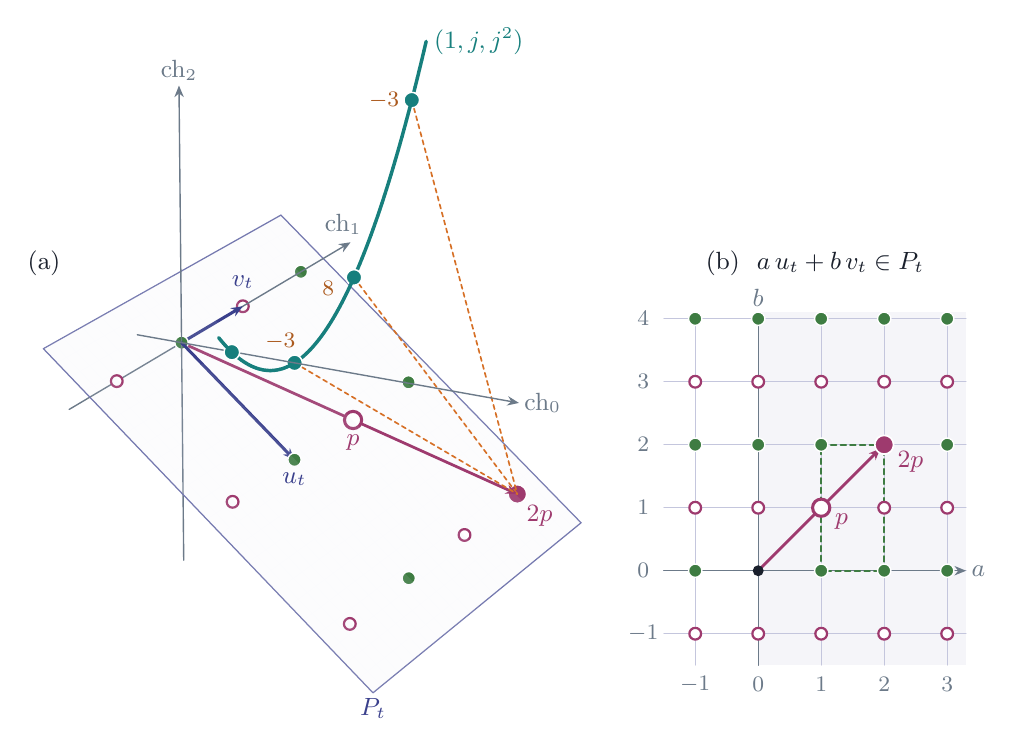
\begin{tikzpicture}[x=1cm,y=1cm,line join=round,line cap=round,
  font=\small,text=PInk]
  \path[draw=none,fill opacity=0.10,fill=PIndigo!16!white] (-0.1816,2.1214) -- (-0.0245,1.9603) -- (0.0761,2.0178) -- (-0.0805,2.1783) -- cycle;
  \path[draw=none,fill opacity=0.10,fill=PIndigo!16!white] (-0.0245,1.9603) -- (0.1328,1.7989) -- (0.2329,1.8570) -- (0.0761,2.0178) -- cycle;
  \path[draw=none,fill opacity=0.10,fill=PIndigo!16!white] (0.1328,1.7989) -- (0.2903,1.6374) -- (0.3899,1.6961) -- (0.2329,1.8570) -- cycle;
  \path[draw=none,fill opacity=0.10,fill=PIndigo!16!white] (0.2903,1.6374) -- (0.4480,1.4757) -- (0.5470,1.5350) -- (0.3899,1.6961) -- cycle;
  \path[draw=none,fill opacity=0.10,fill=PIndigo!16!white] (0.4480,1.4757) -- (0.6059,1.3137) -- (0.7044,1.3737) -- (0.5470,1.5350) -- cycle;
  \path[draw=none,fill opacity=0.10,fill=PIndigo!16!white] (0.6059,1.3137) -- (0.7640,1.1516) -- (0.8620,1.2122) -- (0.7044,1.3737) -- cycle;
  \path[draw=none,fill opacity=0.10,fill=PIndigo!16!white] (-0.2834,2.0642) -- (-0.1258,1.9024) -- (-0.0245,1.9603) -- (-0.1816,2.1214) -- cycle;
  \path[draw=none,fill opacity=0.10,fill=PIndigo!16!white] (0.7640,1.1516) -- (0.9222,0.9892) -- (1.0197,1.0505) -- (0.8620,1.2122) -- cycle;
  \path[draw=none,fill opacity=0.10,fill=PIndigo!16!white] (-0.1258,1.9024) -- (0.0320,1.7404) -- (0.1328,1.7989) -- (-0.0245,1.9603) -- cycle;
  \path[draw=none,fill opacity=0.10,fill=PIndigo!16!white] (0.9222,0.9892) -- (1.0807,0.8267) -- (1.1777,0.8886) -- (1.0197,1.0505) -- cycle;
  \path[draw=none,fill opacity=0.10,fill=PIndigo!16!white] (0.0320,1.7404) -- (0.1900,1.5782) -- (0.2903,1.6374) -- (0.1328,1.7989) -- cycle;
  \path[draw=none,fill opacity=0.10,fill=PIndigo!16!white] (1.0807,0.8267) -- (1.2394,0.6639) -- (1.3358,0.7265) -- (1.1777,0.8886) -- cycle;
  \path[draw=PIndigo!70,line width=0.45pt] (-0.0805,2.1783) -- (3.7314,-1.7293);
  \path[draw=none,fill opacity=0.10,fill=PIndigo!16!white] (0.1900,1.5782) -- (0.3483,1.4159) -- (0.4480,1.4757) -- (0.2903,1.6374) -- cycle;
  \path[draw=none,fill opacity=0.10,fill=PIndigo!16!white] (1.2394,0.6639) -- (1.3982,0.5010) -- (1.4941,0.5641) -- (1.3358,0.7265) -- cycle;
  \path[draw=none,fill opacity=0.10,fill=PIndigo!16!white] (0.3483,1.4159) -- (0.5067,1.2533) -- (0.6059,1.3137) -- (0.4480,1.4757) -- cycle;
  \path[draw=none,fill opacity=0.10,fill=PIndigo!16!white] (1.3982,0.5010) -- (1.5573,0.3379) -- (1.6527,0.4016) -- (1.4941,0.5641) -- cycle;
  \path[draw=none,fill opacity=0.10,fill=PIndigo!16!white] (0.5067,1.2533) -- (0.6653,1.0905) -- (0.7640,1.1516) -- (0.6059,1.3137) -- cycle;
  \path[draw=none,fill opacity=0.10,fill=PIndigo!16!white] (1.5573,0.3379) -- (1.7165,0.1745) -- (1.8114,0.2389) -- (1.6527,0.4016) -- cycle;
  \path[draw=none,fill opacity=0.10,fill=PIndigo!16!white] (-0.3860,2.0065) -- (-0.2278,1.8441) -- (-0.1258,1.9024) -- (-0.2834,2.0642) -- cycle;
  \path[draw=none,fill opacity=0.10,fill=PIndigo!16!white] (0.6653,1.0905) -- (0.8241,0.9275) -- (0.9222,0.9892) -- (0.7640,1.1516) -- cycle;
  \path[draw=none,fill opacity=0.10,fill=PIndigo!16!white] (1.7165,0.1745) -- (1.8760,0.0110) -- (1.9703,0.0760) -- (1.8114,0.2389) -- cycle;
  \path[draw=none,fill opacity=0.10,fill=PIndigo!16!white] (-0.2278,1.8441) -- (-0.0695,1.6815) -- (0.0320,1.7404) -- (-0.1258,1.9024) -- cycle;
  \path[draw=none,fill opacity=0.10,fill=PIndigo!16!white] (0.8241,0.9275) -- (0.9830,0.7644) -- (1.0807,0.8267) -- (0.9222,0.9892) -- cycle;
  \path[draw=none,fill opacity=0.10,fill=PIndigo!16!white] (1.8760,0.0110) -- (2.0356,-0.1528) -- (2.1294,-0.0871) -- (1.9703,0.0760) -- cycle;
  \path[draw=none,fill opacity=0.10,fill=PIndigo!16!white] (-0.0695,1.6815) -- (0.0890,1.5187) -- (0.1900,1.5782) -- (0.0320,1.7404) -- cycle;
  \path[draw=none,fill opacity=0.10,fill=PIndigo!16!white] (0.9830,0.7644) -- (1.1422,0.6010) -- (1.2394,0.6639) -- (1.0807,0.8267) -- cycle;
  \path[draw=none,fill opacity=0.10,fill=PIndigo!16!white] (2.0356,-0.1528) -- (2.1955,-0.3167) -- (2.2887,-0.2504) -- (2.1294,-0.0871) -- cycle;
  \path[draw=none,fill opacity=0.10,fill=PIndigo!16!white] (0.0890,1.5187) -- (0.2478,1.3556) -- (0.3483,1.4159) -- (0.1900,1.5782) -- cycle;
  \path[draw=none,fill opacity=0.10,fill=PIndigo!16!white] (1.1422,0.6010) -- (1.3016,0.4374) -- (1.3982,0.5010) -- (1.2394,0.6639) -- cycle;
  \path[draw=none,fill opacity=0.10,fill=PIndigo!16!white] (2.1955,-0.3167) -- (2.3555,-0.4809) -- (2.4482,-0.4139) -- (2.2887,-0.2504) -- cycle;
  \path[draw=none,fill opacity=0.10,fill=PIndigo!16!white] (0.2478,1.3556) -- (0.4067,1.1924) -- (0.5067,1.2533) -- (0.3483,1.4159) -- cycle;
  \path[draw=none,fill opacity=0.10,fill=PIndigo!16!white] (1.3016,0.4374) -- (1.4612,0.2736) -- (1.5573,0.3379) -- (1.3982,0.5010) -- cycle;
  \path[draw=none,fill opacity=0.10,fill=PIndigo!16!white] (2.3555,-0.4809) -- (2.5158,-0.6453) -- (2.6079,-0.5776) -- (2.4482,-0.4139) -- cycle;
  \node[circle,fill=PGrass,draw=white,line width=0.5pt,inner sep=1.7pt] at (0.1730,1.4583) {};
  \path[draw=none,fill opacity=0.10,fill=PIndigo!16!white] (0.4067,1.1924) -- (0.5658,1.0290) -- (0.6653,1.0905) -- (0.5067,1.2533) -- cycle;
  \path[draw=none,fill opacity=0.10,fill=PIndigo!16!white] (1.4612,0.2736) -- (1.6210,0.1096) -- (1.7165,0.1745) -- (1.5573,0.3379) -- cycle;
  \path[draw=none,fill opacity=0.10,fill=PIndigo!16!white] (2.5158,-0.6453) -- (2.6762,-0.8098) -- (2.7678,-0.7415) -- (2.6079,-0.5776) -- cycle;
  \path[draw=none,fill opacity=0.10,fill=PIndigo!16!white] (-0.4893,1.9484) -- (-0.3306,1.7853) -- (-0.2278,1.8441) -- (-0.3860,2.0065) -- cycle;
  \path[draw=none,fill opacity=0.10,fill=PIndigo!16!white] (0.5658,1.0290) -- (0.7251,0.8654) -- (0.8241,0.9275) -- (0.6653,1.0905) -- cycle;
  \path[draw=none,fill opacity=0.10,fill=PIndigo!16!white] (1.6210,0.1096) -- (1.7810,-0.0546) -- (1.8760,0.0110) -- (1.7165,0.1745) -- cycle;
  \path[draw=none,fill opacity=0.10,fill=PIndigo!16!white] (2.6762,-0.8098) -- (2.8368,-0.9746) -- (2.9279,-0.9056) -- (2.7678,-0.7415) -- cycle;
  \path[draw=none,fill opacity=0.10,fill=PIndigo!16!white] (-0.3306,1.7853) -- (-0.1718,1.6221) -- (-0.0695,1.6815) -- (-0.2278,1.8441) -- cycle;
  \path[draw=none,fill opacity=0.10,fill=PIndigo!16!white] (0.7251,0.8654) -- (0.8847,0.7016) -- (0.9830,0.7644) -- (0.8241,0.9275) -- cycle;
  \path[draw=none,fill opacity=0.10,fill=PIndigo!16!white] (1.7810,-0.0546) -- (1.9411,-0.2190) -- (2.0356,-0.1528) -- (1.8760,0.0110) -- cycle;
  \path[draw=none,fill opacity=0.10,fill=PIndigo!16!white] (2.8368,-0.9746) -- (2.9977,-1.1396) -- (3.0882,-1.0700) -- (2.9279,-0.9056) -- cycle;
  \path[draw=none,fill opacity=0.10,fill=PIndigo!16!white] (-0.1718,1.6221) -- (-0.0127,1.4586) -- (0.0890,1.5187) -- (-0.0695,1.6815) -- cycle;
  \path[draw=none,fill opacity=0.10,fill=PIndigo!16!white] (0.8847,0.7016) -- (1.0444,0.5375) -- (1.1422,0.6010) -- (0.9830,0.7644) -- cycle;
  \path[draw=none,fill opacity=0.10,fill=PIndigo!16!white] (1.9411,-0.2190) -- (2.1015,-0.3836) -- (2.1955,-0.3167) -- (2.0356,-0.1528) -- cycle;
  \path[draw=none,fill opacity=0.10,fill=PIndigo!16!white] (2.9977,-1.1396) -- (3.1587,-1.3047) -- (3.2487,-1.2345) -- (3.0882,-1.0700) -- cycle;
  \path[draw=none,fill opacity=0.10,fill=PIndigo!16!white] (-0.0127,1.4586) -- (0.1465,1.2950) -- (0.2478,1.3556) -- (0.0890,1.5187) -- cycle;
  \path[draw=none,fill opacity=0.10,fill=PIndigo!16!white] (1.0444,0.5375) -- (1.2043,0.3733) -- (1.3016,0.4374) -- (1.1422,0.6010) -- cycle;
  \path[draw=none,fill opacity=0.10,fill=PIndigo!16!white] (2.1015,-0.3836) -- (2.2621,-0.5484) -- (2.3555,-0.4809) -- (2.1955,-0.3167) -- cycle;
  \path[draw=none,fill opacity=0.10,fill=PIndigo!16!white] (3.1587,-1.3047) -- (3.3199,-1.4701) -- (3.4094,-1.3992) -- (3.2487,-1.2345) -- cycle;
  \path[draw=none,fill opacity=0.10,fill=PIndigo!16!white] (0.1465,1.2950) -- (0.3060,1.1311) -- (0.4067,1.1924) -- (0.2478,1.3556) -- cycle;
  \path[draw=none,fill opacity=0.10,fill=PIndigo!16!white] (1.2043,0.3733) -- (1.3644,0.2089) -- (1.4612,0.2736) -- (1.3016,0.4374) -- cycle;
  \path[draw=none,fill opacity=0.10,fill=PIndigo!16!white] (2.2621,-0.5484) -- (2.4229,-0.7134) -- (2.5158,-0.6453) -- (2.3555,-0.4809) -- cycle;
  \path[draw=none,fill opacity=0.10,fill=PIndigo!16!white] (3.3199,-1.4701) -- (3.4814,-1.6357) -- (3.5703,-1.5641) -- (3.4094,-1.3992) -- cycle;
  \path[draw=none,fill opacity=0.10,fill=PIndigo!16!white] (0.3060,1.1311) -- (0.4656,0.9670) -- (0.5658,1.0290) -- (0.4067,1.1924) -- cycle;
  \path[draw=none,fill opacity=0.10,fill=PIndigo!16!white] (1.3644,0.2089) -- (1.5247,0.0442) -- (1.6210,0.1096) -- (1.4612,0.2736) -- cycle;
  \path[draw=none,fill opacity=0.10,fill=PIndigo!16!white] (2.4229,-0.7134) -- (2.5839,-0.8786) -- (2.6762,-0.8098) -- (2.5158,-0.6453) -- cycle;
  \path[draw=none,fill opacity=0.10,fill=PIndigo!16!white] (3.4814,-1.6357) -- (3.6430,-1.8015) -- (3.7314,-1.7293) -- (3.5703,-1.5641) -- cycle;
  \path[draw=none,fill opacity=0.10,fill=PIndigo!16!white] (-0.5934,1.8898) -- (-0.4342,1.7261) -- (-0.3306,1.7853) -- (-0.4893,1.9484) -- cycle;
  \path[draw=none,fill opacity=0.10,fill=PIndigo!16!white] (0.4656,0.9670) -- (0.6255,0.8028) -- (0.7251,0.8654) -- (0.5658,1.0290) -- cycle;
  \path[draw=none,fill opacity=0.10,fill=PIndigo!16!white] (1.5247,0.0442) -- (1.6852,-0.1206) -- (1.7810,-0.0546) -- (1.6210,0.1096) -- cycle;
  \path[draw=none,fill opacity=0.10,fill=PIndigo!16!white] (2.5839,-0.8786) -- (2.7450,-1.0441) -- (2.8368,-0.9746) -- (2.6762,-0.8098) -- cycle;
  \path[draw=none,fill opacity=0.10,fill=PIndigo!16!white] (-0.4342,1.7261) -- (-0.2748,1.5622) -- (-0.1718,1.6221) -- (-0.3306,1.7853) -- cycle;
  \path[draw=none,fill opacity=0.10,fill=PIndigo!16!white] (0.6255,0.8028) -- (0.7855,0.6383) -- (0.8847,0.7016) -- (0.7251,0.8654) -- cycle;
  \path[draw=none,fill opacity=0.10,fill=PIndigo!16!white] (1.6852,-0.1206) -- (1.8460,-0.2857) -- (1.9411,-0.2190) -- (1.7810,-0.0546) -- cycle;
  \path[draw=none,fill opacity=0.10,fill=PIndigo!16!white] (2.7450,-1.0441) -- (2.9064,-1.2097) -- (2.9977,-1.1396) -- (2.8368,-0.9746) -- cycle;
  \node[circle,fill=PGrass,draw=white,line width=0.5pt,inner sep=1.7pt] at (1.5400,0.0546) {};
  \path[draw=none,fill opacity=0.10,fill=PIndigo!16!white] (-0.2748,1.5622) -- (-0.1152,1.3981) -- (-0.0127,1.4586) -- (-0.1718,1.6221) -- cycle;
  \path[draw=none,fill opacity=0.10,fill=PIndigo!16!white] (0.7855,0.6383) -- (0.9458,0.4736) -- (1.0444,0.5375) -- (0.8847,0.7016) -- cycle;
  \path[draw=none,fill opacity=0.10,fill=PIndigo!16!white] (1.8460,-0.2857) -- (2.0069,-0.4509) -- (2.1015,-0.3836) -- (1.9411,-0.2190) -- cycle;
  \path[draw=none,fill opacity=0.10,fill=PIndigo!16!white] (2.9064,-1.2097) -- (3.0680,-1.3755) -- (3.1587,-1.3047) -- (2.9977,-1.1396) -- cycle;
  \path[draw=none,fill opacity=0.10,fill=PIndigo!16!white] (-0.1152,1.3981) -- (0.0445,1.2338) -- (0.1465,1.2950) -- (-0.0127,1.4586) -- cycle;
  \path[draw=none,fill opacity=0.10,fill=PIndigo!16!white] (0.9458,0.4736) -- (1.1063,0.3087) -- (1.2043,0.3733) -- (1.0444,0.5375) -- cycle;
  \path[draw=none,fill opacity=0.10,fill=PIndigo!16!white] (2.0069,-0.4509) -- (2.1680,-0.6164) -- (2.2621,-0.5484) -- (2.1015,-0.3836) -- cycle;
  \path[draw=none,fill opacity=0.10,fill=PIndigo!16!white] (3.0680,-1.3755) -- (3.2298,-1.5416) -- (3.3199,-1.4701) -- (3.1587,-1.3047) -- cycle;
  \path[draw=none,fill opacity=0.10,fill=PIndigo!16!white] (0.0445,1.2338) -- (0.2045,1.0693) -- (0.3060,1.1311) -- (0.1465,1.2950) -- cycle;
  \path[draw=none,fill opacity=0.10,fill=PIndigo!16!white] (1.1063,0.3087) -- (1.2669,0.1436) -- (1.3644,0.2089) -- (1.2043,0.3733) -- cycle;
  \path[draw=none,fill opacity=0.10,fill=PIndigo!16!white] (2.1680,-0.6164) -- (2.3293,-0.7821) -- (2.4229,-0.7134) -- (2.2621,-0.5484) -- cycle;
  \path[draw=none,fill opacity=0.10,fill=PIndigo!16!white] (3.2298,-1.5416) -- (3.3918,-1.7078) -- (3.4814,-1.6357) -- (3.3199,-1.4701) -- cycle;
  \path[draw=none,fill opacity=0.10,fill=PIndigo!16!white] (0.2045,1.0693) -- (0.3647,0.9046) -- (0.4656,0.9670) -- (0.3060,1.1311) -- cycle;
  \path[draw=none,fill opacity=0.10,fill=PIndigo!16!white] (1.2669,0.1436) -- (1.4278,-0.0217) -- (1.5247,0.0442) -- (1.3644,0.2089) -- cycle;
  \path[draw=none,fill opacity=0.10,fill=PIndigo!16!white] (2.3293,-0.7821) -- (2.4908,-0.9480) -- (2.5839,-0.8786) -- (2.4229,-0.7134) -- cycle;
  \path[draw=none,fill opacity=0.10,fill=PIndigo!16!white] (3.3918,-1.7078) -- (3.5539,-1.8743) -- (3.6430,-1.8015) -- (3.4814,-1.6357) -- cycle;
  \path[draw=none,fill opacity=0.10,fill=PIndigo!16!white] (-0.6983,1.8308) -- (-0.5386,1.6665) -- (-0.4342,1.7261) -- (-0.5934,1.8898) -- cycle;
  \path[draw=none,fill opacity=0.10,fill=PIndigo!16!white] (0.3647,0.9046) -- (0.5251,0.7397) -- (0.6255,0.8028) -- (0.4656,0.9670) -- cycle;
  \path[draw=none,fill opacity=0.10,fill=PIndigo!16!white] (1.4278,-0.0217) -- (1.5888,-0.1872) -- (1.6852,-0.1206) -- (1.5247,0.0442) -- cycle;
  \path[draw=none,fill opacity=0.10,fill=PIndigo!16!white] (2.4908,-0.9480) -- (2.6526,-1.1140) -- (2.7450,-1.0441) -- (2.5839,-0.8786) -- cycle;
  \path[draw=none,fill opacity=0.10,fill=PIndigo!16!white] (-0.5386,1.6665) -- (-0.3787,1.5020) -- (-0.2748,1.5622) -- (-0.4342,1.7261) -- cycle;
  \path[draw=none,fill opacity=0.10,fill=PIndigo!16!white] (0.5251,0.7397) -- (0.6857,0.5746) -- (0.7855,0.6383) -- (0.6255,0.8028) -- cycle;
  \path[draw=none,fill opacity=0.10,fill=PIndigo!16!white] (1.5888,-0.1872) -- (1.7501,-0.3529) -- (1.8460,-0.2857) -- (1.6852,-0.1206) -- cycle;
  \path[draw=none,fill opacity=0.10,fill=PIndigo!16!white] (2.6526,-1.1140) -- (2.8145,-1.2803) -- (2.9064,-1.2097) -- (2.7450,-1.0441) -- cycle;
  \path[draw=none,fill opacity=0.10,fill=PIndigo!16!white] (-0.3787,1.5020) -- (-0.2185,1.3372) -- (-0.1152,1.3981) -- (-0.2748,1.5622) -- cycle;
  \path[draw=none,fill opacity=0.10,fill=PIndigo!16!white] (0.6857,0.5746) -- (0.8465,0.4092) -- (0.9458,0.4736) -- (0.7855,0.6383) -- cycle;
  \path[draw=none,fill opacity=0.10,fill=PIndigo!16!white] (1.7501,-0.3529) -- (1.9115,-0.5188) -- (2.0069,-0.4509) -- (1.8460,-0.2857) -- cycle;
  \path[draw=none,fill opacity=0.10,fill=PIndigo!16!white] (2.8145,-1.2803) -- (2.9766,-1.4468) -- (3.0680,-1.3755) -- (2.9064,-1.2097) -- cycle;
  \path[draw=none,fill opacity=0.10,fill=PIndigo!16!white] (-0.2185,1.3372) -- (-0.0582,1.1722) -- (0.0445,1.2338) -- (-0.1152,1.3981) -- cycle;
  \path[draw=none,fill opacity=0.10,fill=PIndigo!16!white] (0.8465,0.4092) -- (1.0075,0.2437) -- (1.1063,0.3087) -- (0.9458,0.4736) -- cycle;
  \path[draw=none,fill opacity=0.10,fill=PIndigo!16!white] (1.9115,-0.5188) -- (2.0732,-0.6849) -- (2.1680,-0.6164) -- (2.0069,-0.4509) -- cycle;
  \path[draw=none,fill opacity=0.10,fill=PIndigo!16!white] (2.9766,-1.4468) -- (3.1389,-1.6135) -- (3.2298,-1.5416) -- (3.0680,-1.3755) -- cycle;
  \path[draw=none,fill opacity=0.10,fill=PIndigo!16!white] (-0.0582,1.1722) -- (0.1023,1.0071) -- (0.2045,1.0693) -- (0.0445,1.2338) -- cycle;
  \path[draw=none,fill opacity=0.10,fill=PIndigo!16!white] (1.0075,0.2437) -- (1.1687,0.0779) -- (1.2669,0.1436) -- (1.1063,0.3087) -- cycle;
  \path[draw=none,fill opacity=0.10,fill=PIndigo!16!white] (2.0732,-0.6849) -- (2.2350,-0.8513) -- (2.3293,-0.7821) -- (2.1680,-0.6164) -- cycle;
  \path[draw=none,fill opacity=0.10,fill=PIndigo!16!white] (3.1389,-1.6135) -- (3.3015,-1.7805) -- (3.3918,-1.7078) -- (3.2298,-1.5416) -- cycle;
  \node[circle,fill=PMag,draw=white,line width=0.6pt,inner sep=2.4pt] at (2.9216,-1.3642) {};
  \path[draw=none,fill opacity=0.10,fill=PIndigo!16!white] (0.1023,1.0071) -- (0.2630,0.8417) -- (0.3647,0.9046) -- (0.2045,1.0693) -- cycle;
  \path[draw=none,fill opacity=0.10,fill=PIndigo!16!white] (1.1687,0.0779) -- (1.3301,-0.0880) -- (1.4278,-0.0217) -- (1.2669,0.1436) -- cycle;
  \path[draw=none,fill opacity=0.10,fill=PIndigo!16!white] (2.2350,-0.8513) -- (2.3971,-1.0178) -- (2.4908,-0.9480) -- (2.3293,-0.7821) -- cycle;
  \path[draw=none,fill opacity=0.10,fill=PIndigo!16!white] (3.3015,-1.7805) -- (3.4642,-1.9476) -- (3.5539,-1.8743) -- (3.3918,-1.7078) -- cycle;
  \path[draw=none,fill opacity=0.10,fill=PIndigo!16!white] (-0.8040,1.7714) -- (-0.6437,1.6064) -- (-0.5386,1.6665) -- (-0.6983,1.8308) -- cycle;
  \path[draw=none,fill opacity=0.10,fill=PIndigo!16!white] (0.2630,0.8417) -- (0.4240,0.6761) -- (0.5251,0.7397) -- (0.3647,0.9046) -- cycle;
  \path[draw=none,fill opacity=0.10,fill=PIndigo!16!white] (1.3301,-0.0880) -- (1.4917,-0.2542) -- (1.5888,-0.1872) -- (1.4278,-0.0217) -- cycle;
  \path[draw=none,fill opacity=0.10,fill=PIndigo!16!white] (2.3971,-1.0178) -- (2.5594,-1.1845) -- (2.6526,-1.1140) -- (2.4908,-0.9480) -- cycle;
  \path[draw=none,fill opacity=0.10,fill=PIndigo!16!white] (-0.6437,1.6064) -- (-0.4833,1.4412) -- (-0.3787,1.5020) -- (-0.5386,1.6665) -- cycle;
  \path[draw=none,fill opacity=0.10,fill=PIndigo!16!white] (0.4240,0.6761) -- (0.5851,0.5103) -- (0.6857,0.5746) -- (0.5251,0.7397) -- cycle;
  \path[draw=none,fill opacity=0.10,fill=PIndigo!16!white] (1.4917,-0.2542) -- (1.6535,-0.4206) -- (1.7501,-0.3529) -- (1.5888,-0.1872) -- cycle;
  \path[draw=none,fill opacity=0.10,fill=PIndigo!16!white] (2.5594,-1.1845) -- (2.7219,-1.3515) -- (2.8145,-1.2803) -- (2.6526,-1.1140) -- cycle;
  \path[draw=none,fill opacity=0.10,fill=PIndigo!16!white] (-0.4833,1.4412) -- (-0.3226,1.2758) -- (-0.2185,1.3372) -- (-0.3787,1.5020) -- cycle;
  \path[draw=none,fill opacity=0.10,fill=PIndigo!16!white] (0.5851,0.5103) -- (0.7464,0.3443) -- (0.8465,0.4092) -- (0.6857,0.5746) -- cycle;
  \path[draw=none,fill opacity=0.10,fill=PIndigo!16!white] (1.6535,-0.4206) -- (1.8155,-0.5872) -- (1.9115,-0.5188) -- (1.7501,-0.3529) -- cycle;
  \path[draw=none,fill opacity=0.10,fill=PIndigo!16!white] (2.7219,-1.3515) -- (2.8845,-1.5187) -- (2.9766,-1.4468) -- (2.8145,-1.2803) -- cycle;
  \path[draw=none,fill opacity=0.10,fill=PIndigo!16!white] (-0.3226,1.2758) -- (-0.1617,1.1102) -- (-0.0582,1.1722) -- (-0.2185,1.3372) -- cycle;
  \path[draw=none,fill opacity=0.10,fill=PIndigo!16!white] (0.7464,0.3443) -- (0.9079,0.1781) -- (1.0075,0.2437) -- (0.8465,0.4092) -- cycle;
  \path[draw=none,fill opacity=0.10,fill=PIndigo!16!white] (1.8155,-0.5872) -- (1.9777,-0.7539) -- (2.0732,-0.6849) -- (1.9115,-0.5188) -- cycle;
  \path[draw=none,fill opacity=0.10,fill=PIndigo!16!white] (2.8845,-1.5187) -- (3.0474,-1.6861) -- (3.1389,-1.6135) -- (2.9766,-1.4468) -- cycle;
  \path[draw=none,fill opacity=0.10,fill=PIndigo!16!white] (-0.1617,1.1102) -- (-0.0007,0.9444) -- (0.1023,1.0071) -- (-0.0582,1.1722) -- cycle;
  \path[draw=none,fill opacity=0.10,fill=PIndigo!16!white] (0.9079,0.1781) -- (1.0697,0.0117) -- (1.1687,0.0779) -- (1.0075,0.2437) -- cycle;
  \path[draw=none,fill opacity=0.10,fill=PIndigo!16!white] (1.9777,-0.7539) -- (2.1401,-0.9210) -- (2.2350,-0.8513) -- (2.0732,-0.6849) -- cycle;
  \path[draw=none,fill opacity=0.10,fill=PIndigo!16!white] (3.0474,-1.6861) -- (3.2105,-1.8537) -- (3.3015,-1.7805) -- (3.1389,-1.6135) -- cycle;
  \path[draw=none,fill opacity=0.10,fill=PIndigo!16!white] (-0.0007,0.9444) -- (0.1606,0.7783) -- (0.2630,0.8417) -- (0.1023,1.0071) -- cycle;
  \path[draw=none,fill opacity=0.10,fill=PIndigo!16!white] (1.0697,0.0117) -- (1.2316,-0.1549) -- (1.3301,-0.0880) -- (1.1687,0.0779) -- cycle;
  \path[draw=none,fill opacity=0.10,fill=PIndigo!16!white] (2.1401,-0.9210) -- (2.3027,-1.0882) -- (2.3971,-1.0178) -- (2.2350,-0.8513) -- cycle;
  \path[draw=none,fill opacity=0.10,fill=PIndigo!16!white] (3.2105,-1.8537) -- (3.3738,-2.0215) -- (3.4642,-1.9476) -- (3.3015,-1.7805) -- cycle;
  \path[draw=none,fill opacity=0.10,fill=PIndigo!16!white] (-0.9104,1.7115) -- (-0.7496,1.5459) -- (-0.6437,1.6064) -- (-0.8040,1.7714) -- cycle;
  \path[draw=none,fill opacity=0.10,fill=PIndigo!16!white] (0.1606,0.7783) -- (0.3220,0.6121) -- (0.4240,0.6761) -- (0.2630,0.8417) -- cycle;
  \path[draw=none,fill opacity=0.10,fill=PIndigo!16!white] (1.2316,-0.1549) -- (1.3938,-0.3217) -- (1.4917,-0.2542) -- (1.3301,-0.0880) -- cycle;
  \path[draw=none,fill opacity=0.10,fill=PIndigo!16!white] (2.3027,-1.0882) -- (2.4655,-1.2556) -- (2.5594,-1.1845) -- (2.3971,-1.0178) -- cycle;
  \path[draw=none,fill opacity=0.10,fill=PIndigo!16!white] (-0.7496,1.5459) -- (-0.5886,1.3800) -- (-0.4833,1.4412) -- (-0.6437,1.6064) -- cycle;
  \path[draw=none,fill opacity=0.10,fill=PIndigo!16!white] (0.3220,0.6121) -- (0.4837,0.4456) -- (0.5851,0.5103) -- (0.4240,0.6761) -- cycle;
  \path[draw=none,fill opacity=0.10,fill=PIndigo!16!white] (1.3938,-0.3217) -- (1.5561,-0.4888) -- (1.6535,-0.4206) -- (1.4917,-0.2542) -- cycle;
  \path[draw=none,fill opacity=0.10,fill=PIndigo!16!white] (2.4655,-1.2556) -- (2.6285,-1.4232) -- (2.7219,-1.3515) -- (2.5594,-1.1845) -- cycle;
  \path[draw=none,fill opacity=0.10,fill=PIndigo!16!white] (-0.5886,1.3800) -- (-0.4274,1.2140) -- (-0.3226,1.2758) -- (-0.4833,1.4412) -- cycle;
  \path[draw=none,fill opacity=0.10,fill=PIndigo!16!white] (0.4837,0.4456) -- (0.6456,0.2790) -- (0.7464,0.3443) -- (0.5851,0.5103) -- cycle;
  \path[draw=none,fill opacity=0.10,fill=PIndigo!16!white] (1.5561,-0.4888) -- (1.7187,-0.6560) -- (1.8155,-0.5872) -- (1.6535,-0.4206) -- cycle;
  \path[draw=none,fill opacity=0.10,fill=PIndigo!16!white] (2.6285,-1.4232) -- (2.7918,-1.5911) -- (2.8845,-1.5187) -- (2.7219,-1.3515) -- cycle;
  \path[draw=none,fill opacity=0.10,fill=PIndigo!16!white] (-0.4274,1.2140) -- (-0.2661,1.0477) -- (-0.1617,1.1102) -- (-0.3226,1.2758) -- cycle;
  \path[draw=none,fill opacity=0.10,fill=PIndigo!16!white] (0.6456,0.2790) -- (0.8077,0.1121) -- (0.9079,0.1781) -- (0.7464,0.3443) -- cycle;
  \path[draw=none,fill opacity=0.10,fill=PIndigo!16!white] (1.7187,-0.6560) -- (1.8814,-0.8235) -- (1.9777,-0.7539) -- (1.8155,-0.5872) -- cycle;
  \path[draw=none,fill opacity=0.10,fill=PIndigo!16!white] (2.7918,-1.5911) -- (2.9552,-1.7591) -- (3.0474,-1.6861) -- (2.8845,-1.5187) -- cycle;
  \path[draw=none,fill opacity=0.10,fill=PIndigo!16!white] (-0.2661,1.0477) -- (-0.1044,0.8812) -- (-0.0007,0.9444) -- (-0.1617,1.1102) -- cycle;
  \path[draw=none,fill opacity=0.10,fill=PIndigo!16!white] (0.8077,0.1121) -- (0.9699,-0.0550) -- (1.0697,0.0117) -- (0.9079,0.1781) -- cycle;
  \path[draw=none,fill opacity=0.10,fill=PIndigo!16!white] (1.8814,-0.8235) -- (2.0444,-0.9912) -- (2.1401,-0.9210) -- (1.9777,-0.7539) -- cycle;
  \path[draw=none,fill opacity=0.10,fill=PIndigo!16!white] (2.9552,-1.7591) -- (3.1189,-1.9274) -- (3.2105,-1.8537) -- (3.0474,-1.6861) -- cycle;
  \path[draw=none,fill opacity=0.10,fill=PIndigo!16!white] (-0.1044,0.8812) -- (0.0574,0.7145) -- (0.1606,0.7783) -- (-0.0007,0.9444) -- cycle;
  \path[draw=none,fill opacity=0.10,fill=PIndigo!16!white] (0.9699,-0.0550) -- (1.1324,-0.2223) -- (1.2316,-0.1549) -- (1.0697,0.0117) -- cycle;
  \path[draw=none,fill opacity=0.10,fill=PIndigo!16!white] (2.0444,-0.9912) -- (2.2076,-1.1591) -- (2.3027,-1.0882) -- (2.1401,-0.9210) -- cycle;
  \path[draw=none,fill opacity=0.10,fill=PIndigo!16!white] (3.1189,-1.9274) -- (3.2827,-2.0959) -- (3.3738,-2.0215) -- (3.2105,-1.8537) -- cycle;
  \path[draw=none,fill opacity=0.10,fill=PIndigo!16!white] (-1.0177,1.6512) -- (-0.8564,1.4849) -- (-0.7496,1.5459) -- (-0.9104,1.7115) -- cycle;
  \path[draw=none,fill opacity=0.10,fill=PIndigo!16!white] (0.0574,0.7145) -- (0.2194,0.5476) -- (0.3220,0.6121) -- (0.1606,0.7783) -- cycle;
  \path[draw=none,fill opacity=0.10,fill=PIndigo!16!white] (1.1324,-0.2223) -- (1.2951,-0.3898) -- (1.3938,-0.3217) -- (1.2316,-0.1549) -- cycle;
  \path[draw=none,fill opacity=0.10,fill=PIndigo!16!white] (2.2076,-1.1591) -- (2.3709,-1.3272) -- (2.4655,-1.2556) -- (2.3027,-1.0882) -- cycle;
  \path[draw=none,fill opacity=0.10,fill=PIndigo!16!white] (-0.8564,1.4849) -- (-0.6948,1.3184) -- (-0.5886,1.3800) -- (-0.7496,1.5459) -- cycle;
  \path[draw=none,fill opacity=0.10,fill=PIndigo!16!white] (0.2194,0.5476) -- (0.3816,0.3805) -- (0.4837,0.4456) -- (0.3220,0.6121) -- cycle;
  \path[draw=none,fill opacity=0.10,fill=PIndigo!16!white] (1.2951,-0.3898) -- (1.4580,-0.5575) -- (1.5561,-0.4888) -- (1.3938,-0.3217) -- cycle;
  \path[draw=none,fill opacity=0.10,fill=PIndigo!16!white] (2.3709,-1.3272) -- (2.5345,-1.4955) -- (2.6285,-1.4232) -- (2.4655,-1.2556) -- cycle;
  \path[draw=none,fill opacity=0.10,fill=PIndigo!16!white] (-0.6948,1.3184) -- (-0.5331,1.1516) -- (-0.4274,1.2140) -- (-0.5886,1.3800) -- cycle;
  \path[draw=none,fill opacity=0.10,fill=PIndigo!16!white] (0.3816,0.3805) -- (0.5440,0.2131) -- (0.6456,0.2790) -- (0.4837,0.4456) -- cycle;
  \path[draw=none,fill opacity=0.10,fill=PIndigo!16!white] (1.4580,-0.5575) -- (1.6211,-0.7254) -- (1.7187,-0.6560) -- (1.5561,-0.4888) -- cycle;
  \path[draw=none,fill opacity=0.10,fill=PIndigo!16!white] (2.5345,-1.4955) -- (2.6983,-1.6640) -- (2.7918,-1.5911) -- (2.6285,-1.4232) -- cycle;
  \draw[PAmber,line width=0.6pt,dash pattern=on 1.6pt off 1.4pt] (1.5813,3.6389) -- (2.9216,-1.3642);
  \path[draw=none,fill opacity=0.10,fill=PIndigo!16!white] (-0.5331,1.1516) -- (-0.3711,0.9847) -- (-0.2661,1.0477) -- (-0.4274,1.2140) -- cycle;
  \path[draw=none,fill opacity=0.10,fill=PIndigo!16!white] (0.5440,0.2131) -- (0.7066,0.0456) -- (0.8077,0.1121) -- (0.6456,0.2790) -- cycle;
  \path[draw=none,fill opacity=0.10,fill=PIndigo!16!white] (1.6211,-0.7254) -- (1.7844,-0.8936) -- (1.8814,-0.8235) -- (1.7187,-0.6560) -- cycle;
  \path[draw=none,fill opacity=0.10,fill=PIndigo!16!white] (2.6983,-1.6640) -- (2.8623,-1.8327) -- (2.9552,-1.7591) -- (2.7918,-1.5911) -- cycle;
  \path[draw=none,fill opacity=0.10,fill=PIndigo!16!white] (-0.3711,0.9847) -- (-0.2090,0.8175) -- (-0.1044,0.8812) -- (-0.2661,1.0477) -- cycle;
  \path[draw=none,fill opacity=0.10,fill=PIndigo!16!white] (0.7066,0.0456) -- (0.8695,-0.1222) -- (0.9699,-0.0550) -- (0.8077,0.1121) -- cycle;
  \path[draw=none,fill opacity=0.10,fill=PIndigo!16!white] (1.7844,-0.8936) -- (1.9480,-1.0619) -- (2.0444,-0.9912) -- (1.8814,-0.8235) -- cycle;
  \path[draw=none,fill opacity=0.10,fill=PIndigo!16!white] (2.8623,-1.8327) -- (3.0265,-2.0017) -- (3.1189,-1.9274) -- (2.9552,-1.7591) -- cycle;
  \path[draw=none,fill opacity=0.10,fill=PIndigo!16!white] (-0.2090,0.8175) -- (-0.0466,0.6502) -- (0.0574,0.7145) -- (-0.1044,0.8812) -- cycle;
  \path[draw=none,fill opacity=0.10,fill=PIndigo!16!white] (0.8695,-0.1222) -- (1.0325,-0.2902) -- (1.1324,-0.2223) -- (0.9699,-0.0550) -- cycle;
  \path[draw=none,fill opacity=0.10,fill=PIndigo!16!white] (1.9480,-1.0619) -- (2.1117,-1.2305) -- (2.2076,-1.1591) -- (2.0444,-0.9912) -- cycle;
  \path[draw=none,fill opacity=0.10,fill=PIndigo!16!white] (3.0265,-2.0017) -- (3.1909,-2.1709) -- (3.2827,-2.0959) -- (3.1189,-1.9274) -- cycle;
  \path[draw=none,fill opacity=0.10,fill=PIndigo!16!white] (-1.1258,1.5904) -- (-0.9639,1.4235) -- (-0.8564,1.4849) -- (-1.0177,1.6512) -- cycle;
  \path[draw=none,fill opacity=0.10,fill=PIndigo!16!white] (-0.0466,0.6502) -- (0.1159,0.4826) -- (0.2194,0.5476) -- (0.0574,0.7145) -- cycle;
  \path[draw=none,fill opacity=0.10,fill=PIndigo!16!white] (1.0325,-0.2902) -- (1.1958,-0.4583) -- (1.2951,-0.3898) -- (1.1324,-0.2223) -- cycle;
  \path[draw=none,fill opacity=0.10,fill=PIndigo!16!white] (2.1117,-1.2305) -- (2.2756,-1.3993) -- (2.3709,-1.3272) -- (2.2076,-1.1591) -- cycle;
  \path[draw=none,fill opacity=0.10,fill=PIndigo!16!white] (-0.9639,1.4235) -- (-0.8018,1.2563) -- (-0.6948,1.3184) -- (-0.8564,1.4849) -- cycle;
  \path[draw=none,fill opacity=0.10,fill=PIndigo!16!white] (0.1159,0.4826) -- (0.2787,0.3148) -- (0.3816,0.3805) -- (0.2194,0.5476) -- cycle;
  \path[draw=none,fill opacity=0.10,fill=PIndigo!16!white] (1.1958,-0.4583) -- (1.3592,-0.6267) -- (1.4580,-0.5575) -- (1.2951,-0.3898) -- cycle;
  \path[draw=none,fill opacity=0.10,fill=PIndigo!16!white] (2.2756,-1.3993) -- (2.4398,-1.5683) -- (2.5345,-1.4955) -- (2.3709,-1.3272) -- cycle;
  \path[draw=none,fill opacity=0.10,fill=PIndigo!16!white] (-0.8018,1.2563) -- (-0.6395,1.0888) -- (-0.5331,1.1516) -- (-0.6948,1.3184) -- cycle;
  \path[draw=none,fill opacity=0.10,fill=PIndigo!16!white] (0.2787,0.3148) -- (0.4416,0.1468) -- (0.5440,0.2131) -- (0.3816,0.3805) -- cycle;
  \path[draw=none,fill opacity=0.10,fill=PIndigo!16!white] (1.3592,-0.6267) -- (1.5229,-0.7954) -- (1.6211,-0.7254) -- (1.4580,-0.5575) -- cycle;
  \path[draw=none,fill opacity=0.10,fill=PIndigo!16!white] (2.4398,-1.5683) -- (2.6041,-1.7375) -- (2.6983,-1.6640) -- (2.5345,-1.4955) -- cycle;
  \path[draw=none,fill opacity=0.10,fill=PIndigo!16!white] (-0.6395,1.0888) -- (-0.4770,0.9212) -- (-0.3711,0.9847) -- (-0.5331,1.1516) -- cycle;
  \path[draw=none,fill opacity=0.10,fill=PIndigo!16!white] (0.4416,0.1468) -- (0.6048,-0.0215) -- (0.7066,0.0456) -- (0.5440,0.2131) -- cycle;
  \path[draw=none,fill opacity=0.10,fill=PIndigo!16!white] (1.5229,-0.7954) -- (1.6867,-0.9642) -- (1.7844,-0.8936) -- (1.6211,-0.7254) -- cycle;
  \path[draw=none,fill opacity=0.10,fill=PIndigo!16!white] (2.6041,-1.7375) -- (2.7687,-1.9069) -- (2.8623,-1.8327) -- (2.6983,-1.6640) -- cycle;
  \path[draw=none,fill opacity=0.10,fill=PIndigo!16!white] (-0.4770,0.9212) -- (-0.3143,0.7534) -- (-0.2090,0.8175) -- (-0.3711,0.9847) -- cycle;
  \path[draw=none,fill opacity=0.10,fill=PIndigo!16!white] (0.6048,-0.0215) -- (0.7682,-0.1899) -- (0.8695,-0.1222) -- (0.7066,0.0456) -- cycle;
  \path[draw=none,fill opacity=0.10,fill=PIndigo!16!white] (1.6867,-0.9642) -- (1.8508,-1.1332) -- (1.9480,-1.0619) -- (1.7844,-0.8936) -- cycle;
  \path[draw=none,fill opacity=0.10,fill=PIndigo!16!white] (2.7687,-1.9069) -- (2.9335,-2.0766) -- (3.0265,-2.0017) -- (2.8623,-1.8327) -- cycle;
  \path[draw=none,fill opacity=0.10,fill=PIndigo!16!white] (-0.3143,0.7534) -- (-0.1514,0.5853) -- (-0.0466,0.6502) -- (-0.2090,0.8175) -- cycle;
  \path[draw=none,fill opacity=0.10,fill=PIndigo!16!white] (0.7682,-0.1899) -- (0.9318,-0.3586) -- (1.0325,-0.2902) -- (0.8695,-0.1222) -- cycle;
  \path[draw=none,fill opacity=0.10,fill=PIndigo!16!white] (1.8508,-1.1332) -- (2.0151,-1.3025) -- (2.1117,-1.2305) -- (1.9480,-1.0619) -- cycle;
  \path[draw=none,fill opacity=0.10,fill=PIndigo!16!white] (2.9335,-2.0766) -- (3.0984,-2.2464) -- (3.1909,-2.1709) -- (3.0265,-2.0017) -- cycle;
  \node[circle,draw=PMag,line width=0.8pt,fill=white,inner sep=1.5pt] at (-0.5643,1.0204) {};
  \path[draw=none,fill opacity=0.10,fill=PIndigo!16!white] (-1.2347,1.5292) -- (-1.0722,1.3615) -- (-0.9639,1.4235) -- (-1.1258,1.5904) -- cycle;
  \path[draw=none,fill opacity=0.10,fill=PIndigo!16!white] (-0.1514,0.5853) -- (0.0117,0.4171) -- (0.1159,0.4826) -- (-0.0466,0.6502) -- cycle;
  \path[draw=none,fill opacity=0.10,fill=PIndigo!16!white] (0.9318,-0.3586) -- (1.0956,-0.5274) -- (1.1958,-0.4583) -- (1.0325,-0.2902) -- cycle;
  \path[draw=none,fill opacity=0.10,fill=PIndigo!16!white] (2.0151,-1.3025) -- (2.1796,-1.4720) -- (2.2756,-1.3993) -- (2.1117,-1.2305) -- cycle;
  \path[draw=none,fill opacity=0.10,fill=PIndigo!16!white] (-1.0722,1.3615) -- (-0.9096,1.1937) -- (-0.8018,1.2563) -- (-0.9639,1.4235) -- cycle;
  \path[draw=none,fill opacity=0.10,fill=PIndigo!16!white] (0.0117,0.4171) -- (0.1750,0.2486) -- (0.2787,0.3148) -- (0.1159,0.4826) -- cycle;
  \path[draw=none,fill opacity=0.10,fill=PIndigo!16!white] (1.0956,-0.5274) -- (1.2596,-0.6965) -- (1.3592,-0.6267) -- (1.1958,-0.4583) -- cycle;
  \path[draw=none,fill opacity=0.10,fill=PIndigo!16!white] (2.1796,-1.4720) -- (2.3443,-1.6416) -- (2.4398,-1.5683) -- (2.2756,-1.3993) -- cycle;
  \draw[PAmber,line width=0.6pt,dash pattern=on 1.6pt off 1.4pt] (0.8471,1.3867) -- (2.9216,-1.3642);
  \path[draw=none,fill opacity=0.10,fill=PIndigo!16!white] (-0.9096,1.1937) -- (-0.7468,1.0256) -- (-0.6395,1.0888) -- (-0.8018,1.2563) -- cycle;
  \path[draw=none,fill opacity=0.10,fill=PIndigo!16!white] (0.1750,0.2486) -- (0.3385,0.0799) -- (0.4416,0.1468) -- (0.2787,0.3148) -- cycle;
  \path[draw=none,fill opacity=0.10,fill=PIndigo!16!white] (1.2596,-0.6965) -- (1.4239,-0.8658) -- (1.5229,-0.7954) -- (1.3592,-0.6267) -- cycle;
  \path[draw=none,fill opacity=0.10,fill=PIndigo!16!white] (2.3443,-1.6416) -- (2.5092,-1.8115) -- (2.6041,-1.7375) -- (2.4398,-1.5683) -- cycle;
  \path[draw=none,fill opacity=0.10,fill=PIndigo!16!white] (-0.7468,1.0256) -- (-0.5837,0.8573) -- (-0.4770,0.9212) -- (-0.6395,1.0888) -- cycle;
  \path[draw=none,fill opacity=0.10,fill=PIndigo!16!white] (0.3385,0.0799) -- (0.5022,-0.0890) -- (0.6048,-0.0215) -- (0.4416,0.1468) -- cycle;
  \path[draw=none,fill opacity=0.10,fill=PIndigo!16!white] (1.4239,-0.8658) -- (1.5883,-1.0353) -- (1.6867,-0.9642) -- (1.5229,-0.7954) -- cycle;
  \path[draw=none,fill opacity=0.10,fill=PIndigo!16!white] (2.5092,-1.8115) -- (2.6744,-1.9817) -- (2.7687,-1.9069) -- (2.6041,-1.7375) -- cycle;
  \path[draw=none,fill opacity=0.10,fill=PIndigo!16!white] (-0.5837,0.8573) -- (-0.4205,0.6887) -- (-0.3143,0.7534) -- (-0.4770,0.9212) -- cycle;
  \path[draw=none,fill opacity=0.10,fill=PIndigo!16!white] (0.5022,-0.0890) -- (0.6662,-0.2581) -- (0.7682,-0.1899) -- (0.6048,-0.0215) -- cycle;
  \path[draw=none,fill opacity=0.10,fill=PIndigo!16!white] (1.5883,-1.0353) -- (1.7529,-1.2051) -- (1.8508,-1.1332) -- (1.6867,-0.9642) -- cycle;
  \path[draw=none,fill opacity=0.10,fill=PIndigo!16!white] (2.6744,-1.9817) -- (2.8397,-2.1520) -- (2.9335,-2.0766) -- (2.7687,-1.9069) -- cycle;
  \draw[PTeal,line width=1.25pt] (1.7361,4.2653) -- (1.7501,4.3246) -- (1.7642,4.3844);
  \path[draw=none,fill opacity=0.10,fill=PIndigo!16!white] (-0.4205,0.6887) -- (-0.2570,0.5200) -- (-0.1514,0.5853) -- (-0.3143,0.7534) -- cycle;
  \path[draw=none,fill opacity=0.10,fill=PIndigo!16!white] (0.6662,-0.2581) -- (0.8303,-0.4275) -- (0.9318,-0.3586) -- (0.7682,-0.1899) -- cycle;
  \path[draw=none,fill opacity=0.10,fill=PIndigo!16!white] (1.7529,-1.2051) -- (1.9178,-1.3750) -- (2.0151,-1.3025) -- (1.8508,-1.1332) -- cycle;
  \path[draw=none,fill opacity=0.10,fill=PIndigo!16!white] (2.8397,-2.1520) -- (3.0052,-2.3226) -- (3.0984,-2.2464) -- (2.9335,-2.0766) -- cycle;
  \draw[PTeal,line width=1.25pt] (1.7081,4.1479) -- (1.7221,4.2064) -- (1.7361,4.2653);
  \draw[PTeal,line width=1.25pt] (1.6800,4.0323) -- (1.6940,4.0899) -- (1.7081,4.1479);
  \path[draw=none,fill opacity=0.10,fill=PIndigo!16!white] (-1.3444,1.4675) -- (-1.1814,1.2991) -- (-1.0722,1.3615) -- (-1.2347,1.5292) -- cycle;
  \path[draw=none,fill opacity=0.10,fill=PIndigo!16!white] (-0.2570,0.5200) -- (-0.0934,0.3511) -- (0.0117,0.4171) -- (-0.1514,0.5853) -- cycle;
  \path[draw=none,fill opacity=0.10,fill=PIndigo!16!white] (0.8303,-0.4275) -- (0.9947,-0.5970) -- (1.0956,-0.5274) -- (0.9318,-0.3586) -- cycle;
  \path[draw=none,fill opacity=0.10,fill=PIndigo!16!white] (1.9178,-1.3750) -- (2.0828,-1.5452) -- (2.1796,-1.4720) -- (2.0151,-1.3025) -- cycle;
  \draw[PTeal,line width=1.25pt] (1.6520,3.9184) -- (1.6660,3.9751) -- (1.6800,4.0323);
  \draw[PTeal,line width=1.25pt] (1.6240,3.8062) -- (1.6380,3.8621) -- (1.6520,3.9184);
  \path[draw=none,fill opacity=0.10,fill=PIndigo!16!white] (-1.1814,1.2991) -- (-1.0183,1.1306) -- (-0.9096,1.1937) -- (-1.0722,1.3615) -- cycle;
  \path[draw=none,fill opacity=0.10,fill=PIndigo!16!white] (-0.0934,0.3511) -- (0.0705,0.1819) -- (0.1750,0.2486) -- (0.0117,0.4171) -- cycle;
  \path[draw=none,fill opacity=0.10,fill=PIndigo!16!white] (0.9947,-0.5970) -- (1.1593,-0.7668) -- (1.2596,-0.6965) -- (1.0956,-0.5274) -- cycle;
  \path[draw=none,fill opacity=0.10,fill=PIndigo!16!white] (2.0828,-1.5452) -- (2.2481,-1.7156) -- (2.3443,-1.6416) -- (2.1796,-1.4720) -- cycle;
  \draw[PTeal,line width=1.25pt] (1.5959,3.6958) -- (1.6099,3.7508) -- (1.6240,3.8062);
  \draw[PTeal,line width=1.25pt] (1.5679,3.5871) -- (1.5819,3.6412) -- (1.5959,3.6958);
  \node[circle,fill=PTeal,draw=white,line width=0.55pt,inner sep=2.0pt] at (1.5813,3.6389) {};
  \path[draw=none,fill opacity=0.10,fill=PIndigo!16!white] (-1.0183,1.1306) -- (-0.8549,0.9618) -- (-0.7468,1.0256) -- (-0.9096,1.1937) -- cycle;
  \path[draw=none,fill opacity=0.10,fill=PIndigo!16!white] (0.0705,0.1819) -- (0.2346,0.0125) -- (0.3385,0.0799) -- (0.1750,0.2486) -- cycle;
  \path[draw=none,fill opacity=0.10,fill=PIndigo!16!white] (1.1593,-0.7668) -- (1.3241,-0.9368) -- (1.4239,-0.8658) -- (1.2596,-0.6965) -- cycle;
  \path[draw=none,fill opacity=0.10,fill=PIndigo!16!white] (2.2481,-1.7156) -- (2.4136,-1.8862) -- (2.5092,-1.8115) -- (2.3443,-1.6416) -- cycle;
  \draw[PMag,line width=1.0pt,-{Stealth[length=4.2pt,width=3.4pt]}] (-1.3425,0.5581) -- (2.9216,-1.3642);
  \node[circle,draw=PMag,line width=1.1pt,fill=white,inner sep=2.2pt] at (0.8357,-0.4238) {};
  \draw[PTeal,line width=1.25pt] (1.5399,3.4801) -- (1.5539,3.5334) -- (1.5679,3.5871);
  \draw[PTeal,line width=1.25pt] (1.5118,3.3749) -- (1.5258,3.4273) -- (1.5399,3.4801);
  \path[draw=none,fill opacity=0.10,fill=PIndigo!16!white] (-0.8549,0.9618) -- (-0.6913,0.7928) -- (-0.5837,0.8573) -- (-0.7468,1.0256) -- cycle;
  \path[draw=none,fill opacity=0.10,fill=PIndigo!16!white] (0.2346,0.0125) -- (0.3989,-0.1571) -- (0.5022,-0.0890) -- (0.3385,0.0799) -- cycle;
  \path[draw=none,fill opacity=0.10,fill=PIndigo!16!white] (1.3241,-0.9368) -- (1.4891,-1.1070) -- (1.5883,-1.0353) -- (1.4239,-0.8658) -- cycle;
  \path[draw=none,fill opacity=0.10,fill=PIndigo!16!white] (2.4136,-1.8862) -- (2.5793,-2.0570) -- (2.6744,-1.9817) -- (2.5092,-1.8115) -- cycle;
  \draw[PTeal,line width=1.25pt] (1.4838,3.2713) -- (1.4978,3.3229) -- (1.5118,3.3749);
  \path[draw=none,fill opacity=0.10,fill=PIndigo!16!white] (-0.6913,0.7928) -- (-0.5275,0.6236) -- (-0.4205,0.6887) -- (-0.5837,0.8573) -- cycle;
  \path[draw=none,fill opacity=0.10,fill=PIndigo!16!white] (0.3989,-0.1571) -- (0.5634,-0.3269) -- (0.6662,-0.2581) -- (0.5022,-0.0890) -- cycle;
  \path[draw=none,fill opacity=0.10,fill=PIndigo!16!white] (1.4891,-1.1070) -- (1.6543,-1.2774) -- (1.7529,-1.2051) -- (1.5883,-1.0353) -- cycle;
  \path[draw=none,fill opacity=0.10,fill=PIndigo!16!white] (2.5793,-2.0570) -- (2.7452,-2.2280) -- (2.8397,-2.1520) -- (2.6744,-1.9817) -- cycle;
  \draw[PTeal,line width=1.25pt] (1.4558,3.1695) -- (1.4698,3.2202) -- (1.4838,3.2713);
  \draw[PTeal,line width=1.25pt] (1.4277,3.0694) -- (1.4417,3.1193) -- (1.4558,3.1695);
  \path[draw=none,fill opacity=0.10,fill=PIndigo!16!white] (-0.5275,0.6236) -- (-0.3634,0.4542) -- (-0.2570,0.5200) -- (-0.4205,0.6887) -- cycle;
  \path[draw=none,fill opacity=0.10,fill=PIndigo!16!white] (0.5634,-0.3269) -- (0.7281,-0.4969) -- (0.8303,-0.4275) -- (0.6662,-0.2581) -- cycle;
  \path[draw=none,fill opacity=0.10,fill=PIndigo!16!white] (1.6543,-1.2774) -- (1.8197,-1.4481) -- (1.9178,-1.3750) -- (1.7529,-1.2051) -- cycle;
  \path[draw=none,fill opacity=0.10,fill=PIndigo!16!white] (2.7452,-2.2280) -- (2.9113,-2.3993) -- (3.0052,-2.3226) -- (2.8397,-2.1520) -- cycle;
  \draw[PTeal,line width=1.25pt] (1.3997,2.9710) -- (1.4137,3.0200) -- (1.4277,3.0694);
  \path[draw=none,fill opacity=0.10,fill=PIndigo!16!white] (-1.4550,1.4053) -- (-1.2914,1.2363) -- (-1.1814,1.2991) -- (-1.3444,1.4675) -- cycle;
  \path[draw=none,fill opacity=0.10,fill=PIndigo!16!white] (-0.3634,0.4542) -- (-0.1992,0.2846) -- (-0.0934,0.3511) -- (-0.2570,0.5200) -- cycle;
  \path[draw=none,fill opacity=0.10,fill=PIndigo!16!white] (0.7281,-0.4969) -- (0.8930,-0.6672) -- (0.9947,-0.5970) -- (0.8303,-0.4275) -- cycle;
  \path[draw=none,fill opacity=0.10,fill=PIndigo!16!white] (1.8197,-1.4481) -- (1.9853,-1.6190) -- (2.0828,-1.5452) -- (1.9178,-1.3750) -- cycle;
  \draw[PTeal,line width=1.25pt] (1.3716,2.8744) -- (1.3857,2.9225) -- (1.3997,2.9710);
  \draw[PTeal,line width=1.25pt] (1.3436,2.7794) -- (1.3576,2.8267) -- (1.3716,2.8744);
  \path[draw=none,fill opacity=0.10,fill=PIndigo!16!white] (-1.2914,1.2363) -- (-1.1277,1.0670) -- (-1.0183,1.1306) -- (-1.1814,1.2991) -- cycle;
  \path[draw=none,fill opacity=0.10,fill=PIndigo!16!white] (-0.1992,0.2846) -- (-0.0348,0.1147) -- (0.0705,0.1819) -- (-0.0934,0.3511) -- cycle;
  \path[draw=none,fill opacity=0.10,fill=PIndigo!16!white] (0.8930,-0.6672) -- (1.0582,-0.8377) -- (1.1593,-0.7668) -- (0.9947,-0.5970) -- cycle;
  \path[draw=none,fill opacity=0.10,fill=PIndigo!16!white] (1.9853,-1.6190) -- (2.1512,-1.7900) -- (2.2481,-1.7156) -- (2.0828,-1.5452) -- cycle;
  \draw[PTeal,line width=1.25pt] (1.3155,2.6862) -- (1.3295,2.7326) -- (1.3436,2.7794);
  \path[draw=none,fill opacity=0.10,fill=PIndigo!16!white] (-1.1277,1.0670) -- (-0.9638,0.8976) -- (-0.8549,0.9618) -- (-1.0183,1.1306) -- cycle;
  \path[draw=none,fill opacity=0.10,fill=PIndigo!16!white] (-0.0348,0.1147) -- (0.1299,-0.0554) -- (0.2346,0.0125) -- (0.0705,0.1819) -- cycle;
  \path[draw=none,fill opacity=0.10,fill=PIndigo!16!white] (1.0582,-0.8377) -- (1.2235,-1.0083) -- (1.3241,-0.9368) -- (1.1593,-0.7668) -- cycle;
  \path[draw=none,fill opacity=0.10,fill=PIndigo!16!white] (2.1512,-1.7900) -- (2.3172,-1.9614) -- (2.4136,-1.8862) -- (2.2481,-1.7156) -- cycle;
  \draw[PTeal,line width=1.25pt] (1.2874,2.5946) -- (1.3015,2.6402) -- (1.3155,2.6862);
  \path[draw=none,fill opacity=0.10,fill=PIndigo!16!white] (-0.9638,0.8976) -- (-0.7996,0.7279) -- (-0.6913,0.7928) -- (-0.8549,0.9618) -- cycle;
  \path[draw=none,fill opacity=0.10,fill=PIndigo!16!white] (0.1299,-0.0554) -- (0.2947,-0.2257) -- (0.3989,-0.1571) -- (0.2346,0.0125) -- cycle;
  \path[draw=none,fill opacity=0.10,fill=PIndigo!16!white] (1.2235,-1.0083) -- (1.3891,-1.1793) -- (1.4891,-1.1070) -- (1.3241,-0.9368) -- cycle;
  \path[draw=none,fill opacity=0.10,fill=PIndigo!16!white] (2.3172,-1.9614) -- (2.4835,-2.1329) -- (2.5793,-2.0570) -- (2.4136,-1.8862) -- cycle;
  \draw[PTeal,line width=1.25pt] (1.2593,2.5048) -- (1.2734,2.5495) -- (1.2874,2.5946);
  \draw[PTeal,line width=1.25pt] (1.2312,2.4166) -- (1.2453,2.4605) -- (1.2593,2.5048);
  \path[draw=none,fill opacity=0.10,fill=PIndigo!16!white] (-0.7996,0.7279) -- (-0.6353,0.5580) -- (-0.5275,0.6236) -- (-0.6913,0.7928) -- cycle;
  \path[draw=none,fill opacity=0.10,fill=PIndigo!16!white] (0.2947,-0.2257) -- (0.4598,-0.3962) -- (0.5634,-0.3269) -- (0.3989,-0.1571) -- cycle;
  \path[draw=none,fill opacity=0.10,fill=PIndigo!16!white] (1.3891,-1.1793) -- (1.5549,-1.3504) -- (1.6543,-1.2774) -- (1.4891,-1.1070) -- cycle;
  \path[draw=none,fill opacity=0.10,fill=PIndigo!16!white] (2.4835,-2.1329) -- (2.6500,-2.3046) -- (2.7452,-2.2280) -- (2.5793,-2.0570) -- cycle;
  \draw[PSlate,line width=0.5pt,-{Stealth[length=4.2pt,width=3.4pt]}] (-2.7694,-0.2894) -- (0.8042,1.8332);
  \draw[PTeal,line width=1.25pt] (1.2031,2.3302) -- (1.2172,2.3732) -- (1.2312,2.4166);
  \node[circle,draw=PMag,line width=0.8pt,fill=white,inner sep=1.5pt] at (2.2512,-1.8840) {};
  \path[draw=none,fill opacity=0.10,fill=PIndigo!16!white] (-0.6353,0.5580) -- (-0.4707,0.3879) -- (-0.3634,0.4542) -- (-0.5275,0.6236) -- cycle;
  \path[draw=none,fill opacity=0.10,fill=PIndigo!16!white] (0.4598,-0.3962) -- (0.6251,-0.5669) -- (0.7281,-0.4969) -- (0.5634,-0.3269) -- cycle;
  \path[draw=none,fill opacity=0.10,fill=PIndigo!16!white] (1.5549,-1.3504) -- (1.7209,-1.5217) -- (1.8197,-1.4481) -- (1.6543,-1.2774) -- cycle;
  \path[draw=none,fill opacity=0.10,fill=PIndigo!16!white] (2.6500,-2.3046) -- (2.8167,-2.4766) -- (2.9113,-2.3993) -- (2.7452,-2.2280) -- cycle;
  \path[draw=PIndigo!70,line width=0.45pt] (-3.0971,0.4818) -- (-0.0805,2.1783);
  \draw[PTeal,line width=1.25pt] (1.1750,2.2455) -- (1.1891,2.2877) -- (1.2031,2.3302);
  \path[draw=none,fill opacity=0.10,fill=PIndigo!16!white] (-1.5664,1.3426) -- (-1.4023,1.1729) -- (-1.2914,1.2363) -- (-1.4550,1.4053) -- cycle;
  \path[draw=none,fill opacity=0.10,fill=PIndigo!16!white] (-0.4707,0.3879) -- (-0.3059,0.2175) -- (-0.1992,0.2846) -- (-0.3634,0.4542) -- cycle;
  \path[draw=none,fill opacity=0.10,fill=PIndigo!16!white] (0.6251,-0.5669) -- (0.7906,-0.7379) -- (0.8930,-0.6672) -- (0.7281,-0.4969) -- cycle;
  \path[draw=none,fill opacity=0.10,fill=PIndigo!16!white] (1.7209,-1.5217) -- (1.8871,-1.6933) -- (1.9853,-1.6190) -- (1.8197,-1.4481) -- cycle;
  \draw[PTeal,line width=1.25pt] (1.1469,2.1625) -- (1.1609,2.2038) -- (1.1750,2.2455);
  \path[draw=none,fill opacity=0.10,fill=PIndigo!16!white] (-1.4023,1.1729) -- (-1.2380,1.0030) -- (-1.1277,1.0670) -- (-1.2914,1.2363) -- cycle;
  \path[draw=none,fill opacity=0.10,fill=PIndigo!16!white] (-0.3059,0.2175) -- (-0.1409,0.0470) -- (-0.0348,0.1147) -- (-0.1992,0.2846) -- cycle;
  \path[draw=none,fill opacity=0.10,fill=PIndigo!16!white] (0.7906,-0.7379) -- (0.9563,-0.9090) -- (1.0582,-0.8377) -- (0.8930,-0.6672) -- cycle;
  \path[draw=none,fill opacity=0.10,fill=PIndigo!16!white] (1.8871,-1.6933) -- (2.0535,-1.8651) -- (2.1512,-1.7900) -- (1.9853,-1.6190) -- cycle;
  \draw[PTeal,line width=1.25pt] (1.1187,2.0812) -- (1.1328,2.1216) -- (1.1469,2.1625);
  \draw[PAmber,line width=0.6pt,dash pattern=on 1.6pt off 1.4pt] (0.0930,0.3018) -- (2.9216,-1.3642);
  \path[draw=none,fill opacity=0.10,fill=PIndigo!16!white] (-1.2380,1.0030) -- (-1.0735,0.8328) -- (-0.9638,0.8976) -- (-1.1277,1.0670) -- cycle;
  \path[draw=none,fill opacity=0.10,fill=PIndigo!16!white] (-0.1409,0.0470) -- (0.0243,-0.1238) -- (0.1299,-0.0554) -- (-0.0348,0.1147) -- cycle;
  \path[draw=none,fill opacity=0.10,fill=PIndigo!16!white] (0.9563,-0.9090) -- (1.1222,-1.0804) -- (1.2235,-1.0083) -- (1.0582,-0.8377) -- cycle;
  \path[draw=none,fill opacity=0.10,fill=PIndigo!16!white] (2.0535,-1.8651) -- (2.2201,-2.0371) -- (2.3172,-1.9614) -- (2.1512,-1.7900) -- cycle;
  \draw[PTeal,line width=1.25pt] (1.0905,2.0016) -- (1.1046,2.0412) -- (1.1187,2.0812);
  \draw[PIndigo,line width=1.1pt,-{Stealth[length=4.2pt,width=3.4pt]}] (-1.3425,0.5581) -- (-0.5643,1.0204);
  \path[draw=none,fill opacity=0.10,fill=PIndigo!16!white] (-1.0735,0.8328) -- (-0.9088,0.6624) -- (-0.7996,0.7279) -- (-0.9638,0.8976) -- cycle;
  \path[draw=none,fill opacity=0.10,fill=PIndigo!16!white] (0.0243,-0.1238) -- (0.1898,-0.2948) -- (0.2947,-0.2257) -- (0.1299,-0.0554) -- cycle;
  \path[draw=none,fill opacity=0.10,fill=PIndigo!16!white] (1.1222,-1.0804) -- (1.2884,-1.2521) -- (1.3891,-1.1793) -- (1.2235,-1.0083) -- cycle;
  \path[draw=none,fill opacity=0.10,fill=PIndigo!16!white] (2.2201,-2.0371) -- (2.3870,-2.2094) -- (2.4835,-2.1329) -- (2.3172,-1.9614) -- cycle;
  \draw[PTeal,line width=1.25pt] (1.0623,1.9237) -- (1.0764,1.9624) -- (1.0905,2.0016);
  \path[draw=none,fill opacity=0.10,fill=PIndigo!16!white] (-0.9088,0.6624) -- (-0.7439,0.4919) -- (-0.6353,0.5580) -- (-0.7996,0.7279) -- cycle;
  \path[draw=none,fill opacity=0.10,fill=PIndigo!16!white] (0.1898,-0.2948) -- (0.3554,-0.4660) -- (0.4598,-0.3962) -- (0.2947,-0.2257) -- cycle;
  \draw[PTeal,line width=1.25pt] (1.0341,1.8475) -- (1.0482,1.8854) -- (1.0623,1.9237);
  \path[draw=none,fill opacity=0.10,fill=PIndigo!16!white] (1.2884,-1.2521) -- (1.4547,-1.4239) -- (1.5549,-1.3504) -- (1.3891,-1.1793) -- cycle;
  \path[draw=none,fill opacity=0.10,fill=PIndigo!16!white] (2.3870,-2.2094) -- (2.5541,-2.3818) -- (2.6500,-2.3046) -- (2.4835,-2.1329) -- cycle;
  \draw[PTeal,line width=1.25pt] (1.0059,1.7730) -- (1.0200,1.8100) -- (1.0341,1.8475);
  \path[draw=none,fill opacity=0.10,fill=PIndigo!16!white] (-0.7439,0.4919) -- (-0.5787,0.3210) -- (-0.4707,0.3879) -- (-0.6353,0.5580) -- cycle;
  \path[draw=none,fill opacity=0.10,fill=PIndigo!16!white] (0.3554,-0.4660) -- (0.5213,-0.6374) -- (0.6251,-0.5669) -- (0.4598,-0.3962) -- cycle;
  \path[draw=none,fill opacity=0.10,fill=PIndigo!16!white] (1.4547,-1.4239) -- (1.6213,-1.5960) -- (1.7209,-1.5217) -- (1.5549,-1.3504) -- cycle;
  \path[draw=none,fill opacity=0.10,fill=PIndigo!16!white] (2.5541,-2.3818) -- (2.7213,-2.5545) -- (2.8167,-2.4766) -- (2.6500,-2.3046) -- cycle;
  \draw[PTeal,line width=1.25pt] (0.9776,1.7002) -- (0.9918,1.7364) -- (1.0059,1.7730);
  \path[draw=none,fill opacity=0.10,fill=PIndigo!16!white] (-1.6787,1.2795) -- (-1.5140,1.1091) -- (-1.4023,1.1729) -- (-1.5664,1.3426) -- cycle;
  \path[draw=none,fill opacity=0.10,fill=PIndigo!16!white] (-0.5787,0.3210) -- (-0.4134,0.1500) -- (-0.3059,0.2175) -- (-0.4707,0.3879) -- cycle;
  \path[draw=none,fill opacity=0.10,fill=PIndigo!16!white] (0.5213,-0.6374) -- (0.6873,-0.8091) -- (0.7906,-0.7379) -- (0.6251,-0.5669) -- cycle;
  \path[draw=none,fill opacity=0.10,fill=PIndigo!16!white] (1.6213,-1.5960) -- (1.7881,-1.7682) -- (1.8871,-1.6933) -- (1.7209,-1.5217) -- cycle;
  \draw[PTeal,line width=1.25pt] (0.9493,1.6291) -- (0.9635,1.6644) -- (0.9776,1.7002);
  \path[draw=none,fill opacity=0.10,fill=PIndigo!16!white] (-1.5140,1.1091) -- (-1.3492,0.9384) -- (-1.2380,1.0030) -- (-1.4023,1.1729) -- cycle;
  \path[draw=none,fill opacity=0.10,fill=PIndigo!16!white] (-0.4134,0.1500) -- (-0.2478,-0.0213) -- (-0.1409,0.0470) -- (-0.3059,0.2175) -- cycle;
  \path[draw=none,fill opacity=0.10,fill=PIndigo!16!white] (0.6873,-0.8091) -- (0.8536,-0.9810) -- (0.9563,-0.9090) -- (0.7906,-0.7379) -- cycle;
  \path[draw=none,fill opacity=0.10,fill=PIndigo!16!white] (1.7881,-1.7682) -- (1.9551,-1.9407) -- (2.0535,-1.8651) -- (1.8871,-1.6933) -- cycle;
  \path[draw=none,fill opacity=0.10,fill=PIndigo!16!white] (-1.3492,0.9384) -- (-1.1841,0.7676) -- (-1.0735,0.8328) -- (-1.2380,1.0030) -- cycle;
  \draw[PTeal,line width=1.25pt] (0.9210,1.5597) -- (0.9352,1.5942) -- (0.9493,1.6291);
  \path[draw=none,fill opacity=0.10,fill=PIndigo!16!white] (-0.2478,-0.0213) -- (-0.0820,-0.1927) -- (0.0243,-0.1238) -- (-0.1409,0.0470) -- cycle;
  \path[draw=none,fill opacity=0.10,fill=PIndigo!16!white] (0.8536,-0.9810) -- (1.0201,-1.1531) -- (1.1222,-1.0804) -- (0.9563,-0.9090) -- cycle;
  \path[draw=none,fill opacity=0.10,fill=PIndigo!16!white] (1.9551,-1.9407) -- (2.1223,-2.1135) -- (2.2201,-2.0371) -- (2.0535,-1.8651) -- cycle;
  \path[draw=none,fill opacity=0.10,fill=PIndigo!16!white] (-1.1841,0.7676) -- (-1.0188,0.5965) -- (-0.9088,0.6624) -- (-1.0735,0.8328) -- cycle;
  \path[draw=none,fill opacity=0.10,fill=PIndigo!16!white] (-0.0820,-0.1927) -- (0.0840,-0.3644) -- (0.1898,-0.2948) -- (0.0243,-0.1238) -- cycle;
  \draw[PTeal,line width=1.25pt] (0.8927,1.4920) -- (0.9069,1.5256) -- (0.9210,1.5597);
  \path[draw=none,fill opacity=0.10,fill=PIndigo!16!white] (1.0201,-1.1531) -- (1.1868,-1.3254) -- (1.2884,-1.2521) -- (1.1222,-1.0804) -- cycle;
  \path[draw=none,fill opacity=0.10,fill=PIndigo!16!white] (2.1223,-2.1135) -- (2.2897,-2.2864) -- (2.3870,-2.2094) -- (2.2201,-2.0371) -- cycle;
  \path[draw=none,fill opacity=0.10,fill=PIndigo!16!white] (-1.0188,0.5965) -- (-0.8533,0.4252) -- (-0.7439,0.4919) -- (-0.9088,0.6624) -- cycle;
  \path[draw=none,fill opacity=0.10,fill=PIndigo!16!white] (0.0840,-0.3644) -- (0.2502,-0.5364) -- (0.3554,-0.4660) -- (0.1898,-0.2948) -- cycle;
  \path[draw=none,fill opacity=0.10,fill=PIndigo!16!white] (1.1868,-1.3254) -- (1.3538,-1.4980) -- (1.4547,-1.4239) -- (1.2884,-1.2521) -- cycle;
  \path[draw=none,fill opacity=0.10,fill=PIndigo!16!white] (2.2897,-2.2864) -- (2.4574,-2.4596) -- (2.5541,-2.3818) -- (2.3870,-2.2094) -- cycle;
  \draw[PTeal,line width=1.25pt] (0.8644,1.4260) -- (0.8785,1.4588) -- (0.8927,1.4920);
  \path[draw=none,fill opacity=0.10,fill=PIndigo!16!white] (-0.8533,0.4252) -- (-0.6876,0.2537) -- (-0.5787,0.3210) -- (-0.7439,0.4919) -- cycle;
  \path[draw=none,fill opacity=0.10,fill=PIndigo!16!white] (0.2502,-0.5364) -- (0.4166,-0.7085) -- (0.5213,-0.6374) -- (0.3554,-0.4660) -- cycle;
  \path[draw=none,fill opacity=0.10,fill=PIndigo!16!white] (1.3538,-1.4980) -- (1.5209,-1.6708) -- (1.6213,-1.5960) -- (1.4547,-1.4239) -- cycle;
  \path[draw=none,fill opacity=0.10,fill=PIndigo!16!white] (2.4574,-2.4596) -- (2.6252,-2.6330) -- (2.7213,-2.5545) -- (2.5541,-2.3818) -- cycle;
  \draw[PTeal,line width=1.25pt] (0.8360,1.3618) -- (0.8502,1.3937) -- (0.8644,1.4260);
  \node[circle,fill=PTeal,draw=white,line width=0.55pt,inner sep=2.0pt] at (0.8471,1.3867) {};
  \path[draw=none,fill opacity=0.10,fill=PIndigo!16!white] (-1.7918,1.2158) -- (-1.6266,1.0447) -- (-1.5140,1.1091) -- (-1.6787,1.2795) -- cycle;
  \path[draw=none,fill opacity=0.10,fill=PIndigo!16!white] (-0.6876,0.2537) -- (-0.5217,0.0819) -- (-0.4134,0.1500) -- (-0.5787,0.3210) -- cycle;
  \path[draw=none,fill opacity=0.10,fill=PIndigo!16!white] (0.4166,-0.7085) -- (0.5833,-0.8809) -- (0.6873,-0.8091) -- (0.5213,-0.6374) -- cycle;
  \path[draw=none,fill opacity=0.10,fill=PIndigo!16!white] (1.5209,-1.6708) -- (1.6883,-1.8438) -- (1.7881,-1.7682) -- (1.6213,-1.5960) -- cycle;
  \draw[PTeal,line width=1.25pt] (0.8076,1.2992) -- (0.8218,1.3303) -- (0.8360,1.3618);
  \path[draw=none,fill opacity=0.10,fill=PIndigo!16!white] (-1.6266,1.0447) -- (-1.4612,0.8734) -- (-1.3492,0.9384) -- (-1.5140,1.1091) -- cycle;
  \path[draw=none,fill opacity=0.10,fill=PIndigo!16!white] (-0.5217,0.0819) -- (-0.3555,-0.0900) -- (-0.2478,-0.0213) -- (-0.4134,0.1500) -- cycle;
  \path[draw=none,fill opacity=0.10,fill=PIndigo!16!white] (0.5833,-0.8809) -- (0.7501,-1.0535) -- (0.8536,-0.9810) -- (0.6873,-0.8091) -- cycle;
  \path[draw=none,fill opacity=0.10,fill=PIndigo!16!white] (1.6883,-1.8438) -- (1.8559,-2.0170) -- (1.9551,-1.9407) -- (1.7881,-1.7682) -- cycle;
  \draw[PTeal,line width=1.25pt] (0.7791,1.2384) -- (0.7933,1.2686) -- (0.8076,1.2992);
  \path[draw=none,fill opacity=0.10,fill=PIndigo!16!white] (-1.4612,0.8734) -- (-1.2956,0.7018) -- (-1.1841,0.7676) -- (-1.3492,0.9384) -- cycle;
  \path[draw=none,fill opacity=0.10,fill=PIndigo!16!white] (-0.3555,-0.0900) -- (-0.1892,-0.2622) -- (-0.0820,-0.1927) -- (-0.2478,-0.0213) -- cycle;
  \path[draw=none,fill opacity=0.10,fill=PIndigo!16!white] (0.7501,-1.0535) -- (0.9172,-1.2263) -- (1.0201,-1.1531) -- (0.8536,-0.9810) -- cycle;
  \path[draw=none,fill opacity=0.10,fill=PIndigo!16!white] (1.8559,-2.0170) -- (2.0237,-2.1904) -- (2.1223,-2.1135) -- (1.9551,-1.9407) -- cycle;
  \draw[PTeal,line width=1.25pt] (0.7506,1.1792) -- (0.7649,1.2086) -- (0.7791,1.2384);
  \path[draw=none,fill opacity=0.10,fill=PIndigo!16!white] (-1.2956,0.7018) -- (-1.1297,0.5300) -- (-1.0188,0.5965) -- (-1.1841,0.7676) -- cycle;
  \path[draw=none,fill opacity=0.10,fill=PIndigo!16!white] (-0.1892,-0.2622) -- (-0.0226,-0.4346) -- (0.0840,-0.3644) -- (-0.0820,-0.1927) -- cycle;
  \path[draw=none,fill opacity=0.10,fill=PIndigo!16!white] (0.9172,-1.2263) -- (1.0845,-1.3994) -- (1.1868,-1.3254) -- (1.0201,-1.1531) -- cycle;
  \path[draw=none,fill opacity=0.10,fill=PIndigo!16!white] (2.0237,-2.1904) -- (2.1917,-2.3641) -- (2.2897,-2.2864) -- (2.1223,-2.1135) -- cycle;
  \draw[PTeal,line width=1.25pt] (0.7221,1.1218) -- (0.7364,1.1503) -- (0.7506,1.1792);
  \path[draw=none,fill opacity=0.10,fill=PIndigo!16!white] (-1.1297,0.5300) -- (-0.9636,0.3580) -- (-0.8533,0.4252) -- (-1.0188,0.5965) -- cycle;
  \path[draw=none,fill opacity=0.10,fill=PIndigo!16!white] (-0.0226,-0.4346) -- (0.1442,-0.6073) -- (0.2502,-0.5364) -- (0.0840,-0.3644) -- cycle;
  \path[draw=none,fill opacity=0.10,fill=PIndigo!16!white] (1.0845,-1.3994) -- (1.2520,-1.5726) -- (1.3538,-1.4980) -- (1.1868,-1.3254) -- cycle;
  \path[draw=none,fill opacity=0.10,fill=PIndigo!16!white] (2.1917,-2.3641) -- (2.3599,-2.5380) -- (2.4574,-2.4596) -- (2.2897,-2.2864) -- cycle;
  \draw[PTeal,line width=1.25pt] (0.6936,1.0661) -- (0.7078,1.0937) -- (0.7221,1.1218);
  \path[draw=none,fill opacity=0.10,fill=PIndigo!16!white] (-0.9636,0.3580) -- (-0.7974,0.1858) -- (-0.6876,0.2537) -- (-0.8533,0.4252) -- cycle;
  \path[draw=none,fill opacity=0.10,fill=PIndigo!16!white] (0.1442,-0.6073) -- (0.3112,-0.7801) -- (0.4166,-0.7085) -- (0.2502,-0.5364) -- cycle;
  \path[draw=none,fill opacity=0.10,fill=PIndigo!16!white] (1.2520,-1.5726) -- (1.4198,-1.7461) -- (1.5209,-1.6708) -- (1.3538,-1.4980) -- cycle;
  \path[draw=none,fill opacity=0.10,fill=PIndigo!16!white] (2.3599,-2.5380) -- (2.5284,-2.7121) -- (2.6252,-2.6330) -- (2.4574,-2.4596) -- cycle;
  \path[draw=none,fill opacity=0.10,fill=PIndigo!16!white] (-1.9059,1.1517) -- (-1.7401,0.9799) -- (-1.6266,1.0447) -- (-1.7918,1.2158) -- cycle;
  \path[draw=none,fill opacity=0.10,fill=PIndigo!16!white] (-0.7974,0.1858) -- (-0.6309,0.0133) -- (-0.5217,0.0819) -- (-0.6876,0.2537) -- cycle;
  \path[draw=none,fill opacity=0.10,fill=PIndigo!16!white] (0.3112,-0.7801) -- (0.4784,-0.9532) -- (0.5833,-0.8809) -- (0.4166,-0.7085) -- cycle;
  \path[draw=none,fill opacity=0.10,fill=PIndigo!16!white] (1.4198,-1.7461) -- (1.5877,-1.9198) -- (1.6883,-1.8438) -- (1.5209,-1.6708) -- cycle;
  \draw[PTeal,line width=1.25pt] (0.6650,1.0121) -- (0.6793,1.0388) -- (0.6936,1.0661);
  \path[draw=none,fill opacity=0.10,fill=PIndigo!16!white] (-1.7401,0.9799) -- (-1.5741,0.8078) -- (-1.4612,0.8734) -- (-1.6266,1.0447) -- cycle;
  \path[draw=none,fill opacity=0.10,fill=PIndigo!16!white] (-0.6309,0.0133) -- (-0.4641,-0.1593) -- (-0.3555,-0.0900) -- (-0.5217,0.0819) -- cycle;
  \path[draw=none,fill opacity=0.10,fill=PIndigo!16!white] (0.4784,-0.9532) -- (0.6459,-1.1266) -- (0.7501,-1.0535) -- (0.5833,-0.8809) -- cycle;
  \path[draw=none,fill opacity=0.10,fill=PIndigo!16!white] (1.5877,-1.9198) -- (1.7559,-2.0938) -- (1.8559,-2.0170) -- (1.6883,-1.8438) -- cycle;
  \draw[PTeal,line width=1.25pt] (0.6364,0.9598) -- (0.6507,0.9857) -- (0.6650,1.0121);
  \path[draw=none,fill opacity=0.10,fill=PIndigo!16!white] (-1.5741,0.8078) -- (-1.4079,0.6356) -- (-1.2956,0.7018) -- (-1.4612,0.8734) -- cycle;
  \path[draw=none,fill opacity=0.10,fill=PIndigo!16!white] (-0.4641,-0.1593) -- (-0.2972,-0.3323) -- (-0.1892,-0.2622) -- (-0.3555,-0.0900) -- cycle;
  \path[draw=none,fill opacity=0.10,fill=PIndigo!16!white] (0.6459,-1.1266) -- (0.8135,-1.3001) -- (0.9172,-1.2263) -- (0.7501,-1.0535) -- cycle;
  \path[draw=none,fill opacity=0.10,fill=PIndigo!16!white] (1.7559,-2.0938) -- (1.9243,-2.2680) -- (2.0237,-2.1904) -- (1.8559,-2.0170) -- cycle;
  \draw[PTeal,line width=1.25pt] (0.6077,0.9092) -- (0.6221,0.9343) -- (0.6364,0.9598);
  \path[draw=none,fill opacity=0.10,fill=PIndigo!16!white] (-1.4079,0.6356) -- (-1.2415,0.4631) -- (-1.1297,0.5300) -- (-1.2956,0.7018) -- cycle;
  \path[draw=none,fill opacity=0.10,fill=PIndigo!16!white] (-0.2972,-0.3323) -- (-0.1300,-0.5054) -- (-0.0226,-0.4346) -- (-0.1892,-0.2622) -- cycle;
  \path[draw=none,fill opacity=0.10,fill=PIndigo!16!white] (0.8135,-1.3001) -- (0.9814,-1.4739) -- (1.0845,-1.3994) -- (0.9172,-1.2263) -- cycle;
  \path[draw=none,fill opacity=0.10,fill=PIndigo!16!white] (1.9243,-2.2680) -- (2.0929,-2.4424) -- (2.1917,-2.3641) -- (2.0237,-2.1904) -- cycle;
  \draw[PTeal,line width=1.25pt] (0.5790,0.8604) -- (0.5934,0.8846) -- (0.6077,0.9092);
  \path[draw=none,fill opacity=0.10,fill=PIndigo!16!white] (-1.2415,0.4631) -- (-1.0748,0.2903) -- (-0.9636,0.3580) -- (-1.1297,0.5300) -- cycle;
  \path[draw=none,fill opacity=0.10,fill=PIndigo!16!white] (-0.1300,-0.5054) -- (0.0373,-0.6787) -- (0.1442,-0.6073) -- (-0.0226,-0.4346) -- cycle;
  \path[draw=none,fill opacity=0.10,fill=PIndigo!16!white] (0.9814,-1.4739) -- (1.1495,-1.6479) -- (1.2520,-1.5726) -- (1.0845,-1.3994) -- cycle;
  \path[draw=none,fill opacity=0.10,fill=PIndigo!16!white] (2.0929,-2.4424) -- (2.2617,-2.6170) -- (2.3599,-2.5380) -- (2.1917,-2.3641) -- cycle;
  \path[draw=none,fill opacity=0.10,fill=PIndigo!16!white] (-1.0748,0.2903) -- (-0.9080,0.1174) -- (-0.7974,0.1858) -- (-0.9636,0.3580) -- cycle;
  \path[draw=none,fill opacity=0.10,fill=PIndigo!16!white] (0.0373,-0.6787) -- (0.2049,-0.8523) -- (0.3112,-0.7801) -- (0.1442,-0.6073) -- cycle;
  \path[draw=none,fill opacity=0.10,fill=PIndigo!16!white] (1.1495,-1.6479) -- (1.3178,-1.8221) -- (1.4198,-1.7461) -- (1.2520,-1.5726) -- cycle;
  \path[draw=none,fill opacity=0.10,fill=PIndigo!16!white] (2.2617,-2.6170) -- (2.4308,-2.7919) -- (2.5284,-2.7121) -- (2.3599,-2.5380) -- cycle;
  \draw[PTeal,line width=1.25pt] (0.5503,0.8132) -- (0.5647,0.8366) -- (0.5790,0.8604);
  \path[draw=PIndigo!70,line width=0.45pt] (1.0888,-3.8883) -- (3.7314,-1.7293);
  \path[draw=none,fill opacity=0.10,fill=PIndigo!16!white] (-2.0208,1.0871) -- (-1.8545,0.9145) -- (-1.7401,0.9799) -- (-1.9059,1.1517) -- cycle;
  \path[draw=none,fill opacity=0.10,fill=PIndigo!16!white] (-0.9080,0.1174) -- (-0.7409,-0.0558) -- (-0.6309,0.0133) -- (-0.7974,0.1858) -- cycle;
  \path[draw=none,fill opacity=0.10,fill=PIndigo!16!white] (0.2049,-0.8523) -- (0.3727,-1.0261) -- (0.4784,-0.9532) -- (0.3112,-0.7801) -- cycle;
  \path[draw=none,fill opacity=0.10,fill=PIndigo!16!white] (1.3178,-1.8221) -- (1.4864,-1.9965) -- (1.5877,-1.9198) -- (1.4198,-1.7461) -- cycle;
  \node[circle,fill=PGrass,draw=white,line width=0.5pt,inner sep=1.7pt] at (-1.3425,0.5581) {};
  \draw[PTeal,line width=1.25pt] (0.5215,0.7678) -- (0.5359,0.7903) -- (0.5503,0.8132);
  \path[draw=none,fill opacity=0.10,fill=PIndigo!16!white] (-1.8545,0.9145) -- (-1.6879,0.7418) -- (-1.5741,0.8078) -- (-1.7401,0.9799) -- cycle;
  \path[draw=none,fill opacity=0.10,fill=PIndigo!16!white] (-0.7409,-0.0558) -- (-0.5736,-0.2292) -- (-0.4641,-0.1593) -- (-0.6309,0.0133) -- cycle;
  \path[draw=none,fill opacity=0.10,fill=PIndigo!16!white] (0.3727,-1.0261) -- (0.5408,-1.2002) -- (0.6459,-1.1266) -- (0.4784,-0.9532) -- cycle;
  \path[draw=none,fill opacity=0.10,fill=PIndigo!16!white] (1.4864,-1.9965) -- (1.6552,-2.1712) -- (1.7559,-2.0938) -- (1.5877,-1.9198) -- cycle;
  \draw[PTeal,line width=1.25pt] (0.4927,0.7242) -- (0.5071,0.7458) -- (0.5215,0.7678);
  \path[draw=none,fill opacity=0.10,fill=PIndigo!16!white] (-1.6879,0.7418) -- (-1.5211,0.5688) -- (-1.4079,0.6356) -- (-1.5741,0.8078) -- cycle;
  \path[draw=none,fill opacity=0.10,fill=PIndigo!16!white] (-0.5736,-0.2292) -- (-0.4061,-0.4028) -- (-0.2972,-0.3323) -- (-0.4641,-0.1593) -- cycle;
  \path[draw=none,fill opacity=0.10,fill=PIndigo!16!white] (0.5408,-1.2002) -- (0.7090,-1.3745) -- (0.8135,-1.3001) -- (0.6459,-1.1266) -- cycle;
  \path[draw=none,fill opacity=0.10,fill=PIndigo!16!white] (1.6552,-2.1712) -- (1.8241,-2.3461) -- (1.9243,-2.2680) -- (1.7559,-2.0938) -- cycle;
  \draw[PSlate,line width=0.5pt,-{Stealth[length=4.2pt,width=3.4pt]}] (-1.3149,-2.2040) -- (-1.3752,3.8238);
  \path[draw=none,fill opacity=0.10,fill=PIndigo!16!white] (-1.5211,0.5688) -- (-1.3541,0.3956) -- (-1.2415,0.4631) -- (-1.4079,0.6356) -- cycle;
  \path[draw=none,fill opacity=0.10,fill=PIndigo!16!white] (-0.4061,-0.4028) -- (-0.2383,-0.5767) -- (-0.1300,-0.5054) -- (-0.2972,-0.3323) -- cycle;
  \path[draw=none,fill opacity=0.10,fill=PIndigo!16!white] (0.7090,-1.3745) -- (0.8775,-1.5490) -- (0.9814,-1.4739) -- (0.8135,-1.3001) -- cycle;
  \path[draw=none,fill opacity=0.10,fill=PIndigo!16!white] (1.8241,-2.3461) -- (1.9933,-2.5213) -- (2.0929,-2.4424) -- (1.9243,-2.2680) -- cycle;
  \draw[PTeal,line width=1.25pt] (0.4638,0.6822) -- (0.4783,0.7030) -- (0.4927,0.7242);
  \path[draw=none,fill opacity=0.10,fill=PIndigo!16!white] (-1.3541,0.3956) -- (-1.1869,0.2221) -- (-1.0748,0.2903) -- (-1.2415,0.4631) -- cycle;
  \path[draw=none,fill opacity=0.10,fill=PIndigo!16!white] (-0.2383,-0.5767) -- (-0.0704,-0.7508) -- (0.0373,-0.6787) -- (-0.1300,-0.5054) -- cycle;
  \path[draw=none,fill opacity=0.10,fill=PIndigo!16!white] (0.8775,-1.5490) -- (1.0462,-1.7237) -- (1.1495,-1.6479) -- (0.9814,-1.4739) -- cycle;
  \path[draw=none,fill opacity=0.10,fill=PIndigo!16!white] (1.9933,-2.5213) -- (2.1628,-2.6966) -- (2.2617,-2.6170) -- (2.0929,-2.4424) -- cycle;
  \draw[PTeal,line width=1.25pt] (0.4349,0.6420) -- (0.4494,0.6619) -- (0.4638,0.6822);
  \draw[PIndigo,line width=1.1pt,-{Stealth[length=4.2pt,width=3.4pt]}] (-1.3425,0.5581) -- (0.0922,-0.9289);
  \path[draw=none,fill opacity=0.10,fill=PIndigo!16!white] (-1.1869,0.2221) -- (-1.0194,0.0484) -- (-0.9080,0.1174) -- (-1.0748,0.2903) -- cycle;
  \path[draw=none,fill opacity=0.10,fill=PIndigo!16!white] (-0.0704,-0.7508) -- (0.0978,-0.9251) -- (0.2049,-0.8523) -- (0.0373,-0.6787) -- cycle;
  \path[draw=none,fill opacity=0.10,fill=PIndigo!16!white] (1.0462,-1.7237) -- (1.2151,-1.8987) -- (1.3178,-1.8221) -- (1.1495,-1.6479) -- cycle;
  \path[draw=none,fill opacity=0.10,fill=PIndigo!16!white] (2.1628,-2.6966) -- (2.3324,-2.8722) -- (2.4308,-2.7919) -- (2.2617,-2.6170) -- cycle;
  \draw[PTeal,line width=1.25pt] (0.4060,0.6036) -- (0.4205,0.6226) -- (0.4349,0.6420);
  \path[draw=none,fill opacity=0.10,fill=PIndigo!16!white] (-2.1366,1.0219) -- (-1.9697,0.8487) -- (-1.8545,0.9145) -- (-2.0208,1.0871) -- cycle;
  \path[draw=none,fill opacity=0.10,fill=PIndigo!16!white] (-1.0194,0.0484) -- (-0.8518,-0.1255) -- (-0.7409,-0.0558) -- (-0.9080,0.1174) -- cycle;
  \path[draw=none,fill opacity=0.10,fill=PIndigo!16!white] (0.0978,-0.9251) -- (0.2662,-1.0996) -- (0.3727,-1.0261) -- (0.2049,-0.8523) -- cycle;
  \path[draw=none,fill opacity=0.10,fill=PIndigo!16!white] (1.2151,-1.8987) -- (1.3842,-2.0738) -- (1.4864,-1.9965) -- (1.3178,-1.8221) -- cycle;
  \path[draw=none,fill opacity=0.10,fill=PIndigo!16!white] (-1.9697,0.8487) -- (-1.8026,0.6752) -- (-1.6879,0.7418) -- (-1.8545,0.9145) -- cycle;
  \path[draw=none,fill opacity=0.10,fill=PIndigo!16!white] (-0.8518,-0.1255) -- (-0.6839,-0.2996) -- (-0.5736,-0.2292) -- (-0.7409,-0.0558) -- cycle;
  \path[draw=none,fill opacity=0.10,fill=PIndigo!16!white] (0.2662,-1.0996) -- (0.4348,-1.2744) -- (0.5408,-1.2002) -- (0.3727,-1.0261) -- cycle;
  \path[draw=none,fill opacity=0.10,fill=PIndigo!16!white] (1.3842,-2.0738) -- (1.5536,-2.2493) -- (1.6552,-2.1712) -- (1.4864,-1.9965) -- cycle;
  \draw[PTeal,line width=1.25pt] (0.3770,0.5669) -- (0.3915,0.5850) -- (0.4060,0.6036);
  \path[draw=none,fill opacity=0.10,fill=PIndigo!16!white] (-1.8026,0.6752) -- (-1.6352,0.5015) -- (-1.5211,0.5688) -- (-1.6879,0.7418) -- cycle;
  \path[draw=none,fill opacity=0.10,fill=PIndigo!16!white] (-0.6839,-0.2996) -- (-0.5158,-0.4740) -- (-0.4061,-0.4028) -- (-0.5736,-0.2292) -- cycle;
  \path[draw=none,fill opacity=0.10,fill=PIndigo!16!white] (0.4348,-1.2744) -- (0.6037,-1.4494) -- (0.7090,-1.3745) -- (0.5408,-1.2002) -- cycle;
  \path[draw=none,fill opacity=0.10,fill=PIndigo!16!white] (1.5536,-2.2493) -- (1.7232,-2.4249) -- (1.8241,-2.3461) -- (1.6552,-2.1712) -- cycle;
  \draw[PTeal,line width=1.25pt] (0.3479,0.5319) -- (0.3625,0.5491) -- (0.3770,0.5669);
  \node[circle,fill=PGrass,draw=white,line width=0.5pt,inner sep=1.7pt] at (0.0922,-0.9289) {};
  \path[draw=none,fill opacity=0.10,fill=PIndigo!16!white] (-1.6352,0.5015) -- (-1.4676,0.3275) -- (-1.3541,0.3956) -- (-1.5211,0.5688) -- cycle;
  \path[draw=none,fill opacity=0.10,fill=PIndigo!16!white] (-0.5158,-0.4740) -- (-0.3474,-0.6485) -- (-0.2383,-0.5767) -- (-0.4061,-0.4028) -- cycle;
  \path[draw=none,fill opacity=0.10,fill=PIndigo!16!white] (0.6037,-1.4494) -- (0.7728,-1.6246) -- (0.8775,-1.5490) -- (0.7090,-1.3745) -- cycle;
  \path[draw=none,fill opacity=0.10,fill=PIndigo!16!white] (1.7232,-2.4249) -- (1.8930,-2.6008) -- (1.9933,-2.5213) -- (1.8241,-2.3461) -- cycle;
  \path[draw=none,fill opacity=0.10,fill=PIndigo!16!white] (-1.4676,0.3275) -- (-1.2998,0.1534) -- (-1.1869,0.2221) -- (-1.3541,0.3956) -- cycle;
  \path[draw=none,fill opacity=0.10,fill=PIndigo!16!white] (-0.3474,-0.6485) -- (-0.1789,-0.8234) -- (-0.0704,-0.7508) -- (-0.2383,-0.5767) -- cycle;
  \path[draw=none,fill opacity=0.10,fill=PIndigo!16!white] (0.7728,-1.6246) -- (0.9420,-1.8001) -- (1.0462,-1.7237) -- (0.8775,-1.5490) -- cycle;
  \path[draw=none,fill opacity=0.10,fill=PIndigo!16!white] (1.8930,-2.6008) -- (2.0630,-2.7769) -- (2.1628,-2.6966) -- (1.9933,-2.5213) -- cycle;
  \draw[PTeal,line width=1.25pt] (0.3188,0.4986) -- (0.3334,0.5150) -- (0.3479,0.5319);
  \path[draw=none,fill opacity=0.10,fill=PIndigo!16!white] (-1.2998,0.1534) -- (-1.1318,-0.0211) -- (-1.0194,0.0484) -- (-1.1869,0.2221) -- cycle;
  \path[draw=none,fill opacity=0.10,fill=PIndigo!16!white] (-0.1789,-0.8234) -- (-0.0101,-0.9984) -- (0.0978,-0.9251) -- (-0.0704,-0.7508) -- cycle;
  \path[draw=none,fill opacity=0.10,fill=PIndigo!16!white] (0.9420,-1.8001) -- (1.1116,-1.9758) -- (1.2151,-1.8987) -- (1.0462,-1.7237) -- cycle;
  \path[draw=none,fill opacity=0.10,fill=PIndigo!16!white] (2.0630,-2.7769) -- (2.2333,-2.9532) -- (2.3324,-2.8722) -- (2.1628,-2.6966) -- cycle;
  \draw[PTeal,line width=1.25pt] (0.2897,0.4672) -- (0.3042,0.4827) -- (0.3188,0.4986);
  \path[draw=none,fill opacity=0.10,fill=PIndigo!16!white] (-2.2534,0.9563) -- (-2.0859,0.7823) -- (-1.9697,0.8487) -- (-2.1366,1.0219) -- cycle;
  \path[draw=none,fill opacity=0.10,fill=PIndigo!16!white] (-1.1318,-0.0211) -- (-0.9635,-0.1957) -- (-0.8518,-0.1255) -- (-1.0194,0.0484) -- cycle;
  \path[draw=none,fill opacity=0.10,fill=PIndigo!16!white] (-0.0101,-0.9984) -- (0.1589,-1.1737) -- (0.2662,-1.0996) -- (0.0978,-0.9251) -- cycle;
  \path[draw=none,fill opacity=0.10,fill=PIndigo!16!white] (1.1116,-1.9758) -- (1.2813,-2.1517) -- (1.3842,-2.0738) -- (1.2151,-1.8987) -- cycle;
  \path[draw=none,fill opacity=0.10,fill=PIndigo!16!white] (-2.0859,0.7823) -- (-1.9181,0.6081) -- (-1.8026,0.6752) -- (-1.9697,0.8487) -- cycle;
  \path[draw=none,fill opacity=0.10,fill=PIndigo!16!white] (-0.9635,-0.1957) -- (-0.7950,-0.3705) -- (-0.6839,-0.2996) -- (-0.8518,-0.1255) -- cycle;
  \path[draw=none,fill opacity=0.10,fill=PIndigo!16!white] (0.1589,-1.1737) -- (0.3281,-1.3492) -- (0.4348,-1.2744) -- (0.2662,-1.0996) -- cycle;
  \path[draw=none,fill opacity=0.10,fill=PIndigo!16!white] (1.2813,-2.1517) -- (1.4513,-2.3279) -- (1.5536,-2.2493) -- (1.3842,-2.0738) -- cycle;
  \draw[PTeal,line width=1.25pt] (0.2605,0.4374) -- (0.2751,0.4521) -- (0.2897,0.4672);
  \path[draw=none,fill opacity=0.10,fill=PIndigo!16!white] (-1.9181,0.6081) -- (-1.7502,0.4336) -- (-1.6352,0.5015) -- (-1.8026,0.6752) -- cycle;
  \path[draw=none,fill opacity=0.10,fill=PIndigo!16!white] (-0.7950,-0.3705) -- (-0.6263,-0.5456) -- (-0.5158,-0.4740) -- (-0.6839,-0.2996) -- cycle;
  \path[draw=none,fill opacity=0.10,fill=PIndigo!16!white] (0.3281,-1.3492) -- (0.4975,-1.5250) -- (0.6037,-1.4494) -- (0.4348,-1.2744) -- cycle;
  \path[draw=none,fill opacity=0.10,fill=PIndigo!16!white] (1.4513,-2.3279) -- (1.6214,-2.5043) -- (1.7232,-2.4249) -- (1.5536,-2.2493) -- cycle;
  \draw[PTeal,line width=1.25pt] (0.2312,0.4095) -- (0.2458,0.4232) -- (0.2605,0.4374);
  \path[draw=none,fill opacity=0.10,fill=PIndigo!16!white] (-1.7502,0.4336) -- (-1.5820,0.2590) -- (-1.4676,0.3275) -- (-1.6352,0.5015) -- cycle;
  \path[draw=none,fill opacity=0.10,fill=PIndigo!16!white] (-0.6263,-0.5456) -- (-0.4574,-0.7210) -- (-0.3474,-0.6485) -- (-0.5158,-0.4740) -- cycle;
  \path[draw=none,fill opacity=0.10,fill=PIndigo!16!white] (0.4975,-1.5250) -- (0.6672,-1.7009) -- (0.7728,-1.6246) -- (0.6037,-1.4494) -- cycle;
  \path[draw=none,fill opacity=0.10,fill=PIndigo!16!white] (1.6214,-2.5043) -- (1.7919,-2.6809) -- (1.8930,-2.6008) -- (1.7232,-2.4249) -- cycle;
  \path[draw=none,fill opacity=0.10,fill=PIndigo!16!white] (-1.5820,0.2590) -- (-1.4136,0.0840) -- (-1.2998,0.1534) -- (-1.4676,0.3275) -- cycle;
  \path[draw=none,fill opacity=0.10,fill=PIndigo!16!white] (-0.4574,-0.7210) -- (-0.2883,-0.8965) -- (-0.1789,-0.8234) -- (-0.3474,-0.6485) -- cycle;
  \path[draw=none,fill opacity=0.10,fill=PIndigo!16!white] (0.6672,-1.7009) -- (0.8371,-1.8771) -- (0.9420,-1.8001) -- (0.7728,-1.6246) -- cycle;
  \path[draw=none,fill opacity=0.10,fill=PIndigo!16!white] (1.7919,-2.6809) -- (1.9625,-2.8578) -- (2.0630,-2.7769) -- (1.8930,-2.6008) -- cycle;
  \draw[PTeal,line width=1.25pt] (0.2019,0.3833) -- (0.2165,0.3961) -- (0.2312,0.4095);
  \path[draw=none,fill opacity=0.10,fill=PIndigo!16!white] (-1.4136,0.0840) -- (-1.2450,-0.0911) -- (-1.1318,-0.0211) -- (-1.2998,0.1534) -- cycle;
  \path[draw=none,fill opacity=0.10,fill=PIndigo!16!white] (-0.2883,-0.8965) -- (-0.1189,-1.0723) -- (-0.0101,-0.9984) -- (-0.1789,-0.8234) -- cycle;
  \path[draw=none,fill opacity=0.10,fill=PIndigo!16!white] (0.8371,-1.8771) -- (1.0072,-2.0536) -- (1.1116,-1.9758) -- (0.9420,-1.8001) -- cycle;
  \path[draw=none,fill opacity=0.10,fill=PIndigo!16!white] (1.9625,-2.8578) -- (2.1334,-3.0349) -- (2.2333,-2.9532) -- (2.0630,-2.7769) -- cycle;
  \node[circle,fill=PGrass,draw=white,line width=0.5pt,inner sep=1.7pt] at (1.5431,-2.4329) {};
  \draw[PTeal,line width=1.25pt] (0.1725,0.3588) -- (0.1872,0.3708) -- (0.2019,0.3833);
  \path[draw=none,fill opacity=0.10,fill=PIndigo!16!white] (-2.3710,0.8901) -- (-2.2029,0.7154) -- (-2.0859,0.7823) -- (-2.2534,0.9563) -- cycle;
  \path[draw=none,fill opacity=0.10,fill=PIndigo!16!white] (-1.2450,-0.0911) -- (-1.0762,-0.2665) -- (-0.9635,-0.1957) -- (-1.1318,-0.0211) -- cycle;
  \path[draw=none,fill opacity=0.10,fill=PIndigo!16!white] (-0.1189,-1.0723) -- (0.0507,-1.2483) -- (0.1589,-1.1737) -- (-0.0101,-0.9984) -- cycle;
  \path[draw=none,fill opacity=0.10,fill=PIndigo!16!white] (1.0072,-2.0536) -- (1.1775,-2.2303) -- (1.2813,-2.1517) -- (1.1116,-1.9758) -- cycle;
  \path[draw=none,fill opacity=0.10,fill=PIndigo!16!white] (-2.2029,0.7154) -- (-2.0346,0.5404) -- (-1.9181,0.6081) -- (-2.0859,0.7823) -- cycle;
  \path[draw=none,fill opacity=0.10,fill=PIndigo!16!white] (-1.0762,-0.2665) -- (-0.9071,-0.4421) -- (-0.7950,-0.3705) -- (-0.9635,-0.1957) -- cycle;
  \path[draw=none,fill opacity=0.10,fill=PIndigo!16!white] (0.0507,-1.2483) -- (0.2205,-1.4246) -- (0.3281,-1.3492) -- (0.1589,-1.1737) -- cycle;
  \path[draw=none,fill opacity=0.10,fill=PIndigo!16!white] (1.1775,-2.2303) -- (1.3481,-2.4072) -- (1.4513,-2.3279) -- (1.2813,-2.1517) -- cycle;
  \draw[PTeal,line width=1.25pt] (0.1431,0.3362) -- (0.1578,0.3473) -- (0.1725,0.3588);
  \path[draw=none,fill opacity=0.10,fill=PIndigo!16!white] (-2.0346,0.5404) -- (-1.8661,0.3653) -- (-1.7502,0.4336) -- (-1.9181,0.6081) -- cycle;
  \path[draw=none,fill opacity=0.10,fill=PIndigo!16!white] (-0.9071,-0.4421) -- (-0.7378,-0.6179) -- (-0.6263,-0.5456) -- (-0.7950,-0.3705) -- cycle;
  \path[draw=none,fill opacity=0.10,fill=PIndigo!16!white] (0.2205,-1.4246) -- (0.3905,-1.6011) -- (0.4975,-1.5250) -- (0.3281,-1.3492) -- cycle;
  \path[draw=none,fill opacity=0.10,fill=PIndigo!16!white] (1.3481,-2.4072) -- (1.5189,-2.5843) -- (1.6214,-2.5043) -- (1.4513,-2.3279) -- cycle;
  \draw[PTeal,line width=1.25pt] (0.1136,0.3153) -- (0.1283,0.3255) -- (0.1431,0.3362);
  \path[draw=none,fill opacity=0.10,fill=PIndigo!16!white] (-1.8661,0.3653) -- (-1.6973,0.1898) -- (-1.5820,0.2590) -- (-1.7502,0.4336) -- cycle;
  \path[draw=none,fill opacity=0.10,fill=PIndigo!16!white] (-0.7378,-0.6179) -- (-0.5683,-0.7940) -- (-0.4574,-0.7210) -- (-0.6263,-0.5456) -- cycle;
  \path[draw=none,fill opacity=0.10,fill=PIndigo!16!white] (0.3905,-1.6011) -- (0.5608,-1.7778) -- (0.6672,-1.7009) -- (0.4975,-1.5250) -- cycle;
  \path[draw=none,fill opacity=0.10,fill=PIndigo!16!white] (1.5189,-2.5843) -- (1.6899,-2.7617) -- (1.7919,-2.6809) -- (1.6214,-2.5043) -- cycle;
  \path[draw=none,fill opacity=0.10,fill=PIndigo!16!white] (-1.6973,0.1898) -- (-1.5283,0.0142) -- (-1.4136,0.0840) -- (-1.5820,0.2590) -- cycle;
  \path[draw=none,fill opacity=0.10,fill=PIndigo!16!white] (-0.5683,-0.7940) -- (-0.3985,-0.9703) -- (-0.2883,-0.8965) -- (-0.4574,-0.7210) -- cycle;
  \path[draw=none,fill opacity=0.10,fill=PIndigo!16!white] (0.5608,-1.7778) -- (0.7313,-1.9548) -- (0.8371,-1.8771) -- (0.6672,-1.7009) -- cycle;
  \path[draw=none,fill opacity=0.10,fill=PIndigo!16!white] (1.6899,-2.7617) -- (1.8612,-2.9393) -- (1.9625,-2.8578) -- (1.7919,-2.6809) -- cycle;
  \draw[PTeal,line width=1.25pt] (0.0840,0.2962) -- (0.0988,0.3055) -- (0.1136,0.3153);
  \node[circle,fill=PTeal,draw=white,line width=0.55pt,inner sep=2.0pt] at (0.0930,0.3018) {};
  \path[draw=none,fill opacity=0.10,fill=PIndigo!16!white] (-1.5283,0.0142) -- (-1.3591,-0.1617) -- (-1.2450,-0.0911) -- (-1.4136,0.0840) -- cycle;
  \path[draw=none,fill opacity=0.10,fill=PIndigo!16!white] (-0.3985,-0.9703) -- (-0.2286,-1.1468) -- (-0.1189,-1.0723) -- (-0.2883,-0.8965) -- cycle;
  \path[draw=none,fill opacity=0.10,fill=PIndigo!16!white] (0.7313,-1.9548) -- (0.9020,-2.1320) -- (1.0072,-2.0536) -- (0.8371,-1.8771) -- cycle;
  \path[draw=none,fill opacity=0.10,fill=PIndigo!16!white] (1.8612,-2.9393) -- (2.0326,-3.1172) -- (2.1334,-3.0349) -- (1.9625,-2.8578) -- cycle;
  \path[draw=none,fill opacity=0.10,fill=PIndigo!16!white] (-2.4896,0.8234) -- (-2.3210,0.6480) -- (-2.2029,0.7154) -- (-2.3710,0.8901) -- cycle;
  \path[draw=none,fill opacity=0.10,fill=PIndigo!16!white] (-1.3591,-0.1617) -- (-1.1897,-0.3378) -- (-1.0762,-0.2665) -- (-1.2450,-0.0911) -- cycle;
  \path[draw=none,fill opacity=0.10,fill=PIndigo!16!white] (-0.2286,-1.1468) -- (-0.0584,-1.3236) -- (0.0507,-1.2483) -- (-0.1189,-1.0723) -- cycle;
  \path[draw=none,fill opacity=0.10,fill=PIndigo!16!white] (0.9020,-2.1320) -- (1.0730,-2.3094) -- (1.1775,-2.2303) -- (1.0072,-2.0536) -- cycle;
  \draw[PTeal,line width=1.25pt] (0.0544,0.2788) -- (0.0692,0.2873) -- (0.0840,0.2962);
  \path[draw=none,fill opacity=0.10,fill=PIndigo!16!white] (-2.3210,0.6480) -- (-2.1521,0.4723) -- (-2.0346,0.5404) -- (-2.2029,0.7154) -- cycle;
  \path[draw=none,fill opacity=0.10,fill=PIndigo!16!white] (-1.1897,-0.3378) -- (-1.0200,-0.5142) -- (-0.9071,-0.4421) -- (-1.0762,-0.2665) -- cycle;
  \path[draw=none,fill opacity=0.10,fill=PIndigo!16!white] (-0.0584,-1.3236) -- (0.1120,-1.5006) -- (0.2205,-1.4246) -- (0.0507,-1.2483) -- cycle;
  \path[draw=none,fill opacity=0.10,fill=PIndigo!16!white] (1.0730,-2.3094) -- (1.2441,-2.4871) -- (1.3481,-2.4072) -- (1.1775,-2.2303) -- cycle;
  \draw[PTeal,line width=1.25pt] (0.0247,0.2633) -- (0.0396,0.2708) -- (0.0544,0.2788);
  \path[draw=none,fill opacity=0.10,fill=PIndigo!16!white] (-2.1521,0.4723) -- (-1.9829,0.2963) -- (-1.8661,0.3653) -- (-2.0346,0.5404) -- cycle;
  \path[draw=none,fill opacity=0.10,fill=PIndigo!16!white] (-1.0200,-0.5142) -- (-0.8501,-0.6907) -- (-0.7378,-0.6179) -- (-0.9071,-0.4421) -- cycle;
  \path[draw=none,fill opacity=0.10,fill=PIndigo!16!white] (0.1120,-1.5006) -- (0.2827,-1.6778) -- (0.3905,-1.6011) -- (0.2205,-1.4246) -- cycle;
  \path[draw=none,fill opacity=0.10,fill=PIndigo!16!white] (1.2441,-2.4871) -- (1.4155,-2.6650) -- (1.5189,-2.5843) -- (1.3481,-2.4072) -- cycle;
  \path[draw=none,fill opacity=0.10,fill=PIndigo!16!white] (-1.9829,0.2963) -- (-1.8136,0.1202) -- (-1.6973,0.1898) -- (-1.8661,0.3653) -- cycle;
  \path[draw=none,fill opacity=0.10,fill=PIndigo!16!white] (-0.8501,-0.6907) -- (-0.6800,-0.8676) -- (-0.5683,-0.7940) -- (-0.7378,-0.6179) -- cycle;
  \path[draw=none,fill opacity=0.10,fill=PIndigo!16!white] (0.2827,-1.6778) -- (0.4535,-1.8553) -- (0.5608,-1.7778) -- (0.3905,-1.6011) -- cycle;
  \path[draw=none,fill opacity=0.10,fill=PIndigo!16!white] (1.4155,-2.6650) -- (1.5872,-2.8431) -- (1.6899,-2.7617) -- (1.5189,-2.5843) -- cycle;
  \draw[PTeal,line width=1.25pt] (-0.0050,0.2496) -- (0.0098,0.2562) -- (0.0247,0.2633);
  \path[draw=none,fill opacity=0.10,fill=PIndigo!16!white] (-1.8136,0.1202) -- (-1.6440,-0.0562) -- (-1.5283,0.0142) -- (-1.6973,0.1898) -- cycle;
  \path[draw=none,fill opacity=0.10,fill=PIndigo!16!white] (-0.6800,-0.8676) -- (-0.5097,-1.0446) -- (-0.3985,-0.9703) -- (-0.5683,-0.7940) -- cycle;
  \path[draw=none,fill opacity=0.10,fill=PIndigo!16!white] (0.4535,-1.8553) -- (0.6246,-2.0330) -- (0.7313,-1.9548) -- (0.5608,-1.7778) -- cycle;
  \path[draw=none,fill opacity=0.10,fill=PIndigo!16!white] (1.5872,-2.8431) -- (1.7590,-3.0215) -- (1.8612,-2.9393) -- (1.6899,-2.7617) -- cycle;
  \draw[PSlate,line width=0.5pt,-{Stealth[length=4.2pt,width=3.4pt]}] (-1.9049,0.6586) -- (2.9424,-0.2071);
  \path[draw=none,fill opacity=0.10,fill=PIndigo!16!white] (-1.6440,-0.0562) -- (-1.4742,-0.2328) -- (-1.3591,-0.1617) -- (-1.5283,0.0142) -- cycle;
  \path[draw=none,fill opacity=0.10,fill=PIndigo!16!white] (-0.5097,-1.0446) -- (-0.3391,-1.2219) -- (-0.2286,-1.1468) -- (-0.3985,-0.9703) -- cycle;
  \path[draw=none,fill opacity=0.10,fill=PIndigo!16!white] (0.6246,-2.0330) -- (0.7960,-2.2110) -- (0.9020,-2.1320) -- (0.7313,-1.9548) -- cycle;
  \path[draw=none,fill opacity=0.10,fill=PIndigo!16!white] (1.7590,-3.0215) -- (1.9311,-3.2001) -- (2.0326,-3.1172) -- (1.8612,-2.9393) -- cycle;
  \draw[PTeal,line width=1.25pt] (-0.0349,0.2376) -- (-0.0199,0.2434) -- (-0.0050,0.2496);
  \path[draw=none,fill opacity=0.10,fill=PIndigo!16!white] (-2.6092,0.7562) -- (-2.4399,0.5800) -- (-2.3210,0.6480) -- (-2.4896,0.8234) -- cycle;
  \path[draw=none,fill opacity=0.10,fill=PIndigo!16!white] (-1.4742,-0.2328) -- (-1.3041,-0.4097) -- (-1.1897,-0.3378) -- (-1.3591,-0.1617) -- cycle;
  \path[draw=none,fill opacity=0.10,fill=PIndigo!16!white] (-0.3391,-1.2219) -- (-0.1683,-1.3994) -- (-0.0584,-1.3236) -- (-0.2286,-1.1468) -- cycle;
  \path[draw=none,fill opacity=0.10,fill=PIndigo!16!white] (0.7960,-2.2110) -- (0.9675,-2.3892) -- (1.0730,-2.3094) -- (0.9020,-2.1320) -- cycle;
  \path[draw=none,fill opacity=0.10,fill=PIndigo!16!white] (-2.4399,0.5800) -- (-2.2704,0.4035) -- (-2.1521,0.4723) -- (-2.3210,0.6480) -- cycle;
  \draw[PTeal,line width=1.25pt] (-0.0647,0.2275) -- (-0.0498,0.2324) -- (-0.0349,0.2376);
  \path[draw=none,fill opacity=0.10,fill=PIndigo!16!white] (-1.3041,-0.4097) -- (-1.1339,-0.5868) -- (-1.0200,-0.5142) -- (-1.1897,-0.3378) -- cycle;
  \path[draw=none,fill opacity=0.10,fill=PIndigo!16!white] (-0.1683,-1.3994) -- (0.0027,-1.5772) -- (0.1120,-1.5006) -- (-0.0584,-1.3236) -- cycle;
  \path[draw=none,fill opacity=0.10,fill=PIndigo!16!white] (0.9675,-2.3892) -- (1.1393,-2.5676) -- (1.2441,-2.4871) -- (1.0730,-2.3094) -- cycle;
  \path[draw=none,fill opacity=0.10,fill=PIndigo!16!white] (-2.2704,0.4035) -- (-2.1007,0.2269) -- (-1.9829,0.2963) -- (-2.1521,0.4723) -- cycle;
  \path[draw=none,fill opacity=0.10,fill=PIndigo!16!white] (-1.1339,-0.5868) -- (-0.9634,-0.7642) -- (-0.8501,-0.6907) -- (-1.0200,-0.5142) -- cycle;
  \path[draw=none,fill opacity=0.10,fill=PIndigo!16!white] (0.0027,-1.5772) -- (0.1740,-1.7552) -- (0.2827,-1.6778) -- (0.1120,-1.5006) -- cycle;
  \path[draw=none,fill opacity=0.10,fill=PIndigo!16!white] (1.1393,-2.5676) -- (1.3113,-2.7463) -- (1.4155,-2.6650) -- (1.2441,-2.4871) -- cycle;
  \draw[PTeal,line width=1.25pt] (-0.0947,0.2192) -- (-0.0797,0.2231) -- (-0.0647,0.2275);
  \path[draw=none,fill opacity=0.10,fill=PIndigo!16!white] (-2.1007,0.2269) -- (-1.9307,0.0500) -- (-1.8136,0.1202) -- (-1.9829,0.2963) -- cycle;
  \path[draw=none,fill opacity=0.10,fill=PIndigo!16!white] (-0.9634,-0.7642) -- (-0.7927,-0.9417) -- (-0.6800,-0.8676) -- (-0.8501,-0.6907) -- cycle;
  \path[draw=none,fill opacity=0.10,fill=PIndigo!16!white] (0.1740,-1.7552) -- (0.3454,-1.9334) -- (0.4535,-1.8553) -- (0.2827,-1.6778) -- cycle;
  \path[draw=none,fill opacity=0.10,fill=PIndigo!16!white] (1.3113,-2.7463) -- (1.4836,-2.9252) -- (1.5872,-2.8431) -- (1.4155,-2.6650) -- cycle;
  \path[draw=none,fill opacity=0.10,fill=PIndigo!16!white] (-1.9307,0.0500) -- (-1.7605,-0.1272) -- (-1.6440,-0.0562) -- (-1.8136,0.1202) -- cycle;
  \path[draw=none,fill opacity=0.10,fill=PIndigo!16!white] (-0.7927,-0.9417) -- (-0.6217,-1.1195) -- (-0.5097,-1.0446) -- (-0.6800,-0.8676) -- cycle;
  \path[draw=none,fill opacity=0.10,fill=PIndigo!16!white] (0.3454,-1.9334) -- (0.5171,-2.1119) -- (0.6246,-2.0330) -- (0.4535,-1.8553) -- cycle;
  \path[draw=none,fill opacity=0.10,fill=PIndigo!16!white] (1.4836,-2.9252) -- (1.6561,-3.1043) -- (1.7590,-3.0215) -- (1.5872,-2.8431) -- cycle;
  \draw[PTeal,line width=1.25pt] (-0.1247,0.2127) -- (-0.1097,0.2157) -- (-0.0947,0.2192);
  \path[draw=none,fill opacity=0.10,fill=PIndigo!16!white] (-1.7605,-0.1272) -- (-1.5901,-0.3046) -- (-1.4742,-0.2328) -- (-1.6440,-0.0562) -- cycle;
  \path[draw=none,fill opacity=0.10,fill=PIndigo!16!white] (-0.6217,-1.1195) -- (-0.4505,-1.2976) -- (-0.3391,-1.2219) -- (-0.5097,-1.0446) -- cycle;
  \path[draw=none,fill opacity=0.10,fill=PIndigo!16!white] (0.5171,-2.1119) -- (0.6891,-2.2906) -- (0.7960,-2.2110) -- (0.6246,-2.0330) -- cycle;
  \path[draw=none,fill opacity=0.10,fill=PIndigo!16!white] (1.6561,-3.1043) -- (1.8288,-3.2837) -- (1.9311,-3.2001) -- (1.7590,-3.0215) -- cycle;
  \path[draw=none,fill opacity=0.10,fill=PIndigo!16!white] (-2.7297,0.6884) -- (-2.5598,0.5115) -- (-2.4399,0.5800) -- (-2.6092,0.7562) -- cycle;
  \path[draw=none,fill opacity=0.10,fill=PIndigo!16!white] (-1.5901,-0.3046) -- (-1.4195,-0.4822) -- (-1.3041,-0.4097) -- (-1.4742,-0.2328) -- cycle;
  \path[draw=none,fill opacity=0.10,fill=PIndigo!16!white] (-0.4505,-1.2976) -- (-0.2791,-1.4759) -- (-0.1683,-1.3994) -- (-0.3391,-1.2219) -- cycle;
  \path[draw=none,fill opacity=0.10,fill=PIndigo!16!white] (0.6891,-2.2906) -- (0.8613,-2.4696) -- (0.9675,-2.3892) -- (0.7960,-2.2110) -- cycle;
  \draw[PTeal,line width=1.25pt] (-0.1548,0.2081) -- (-0.1398,0.2102) -- (-0.1247,0.2127);
  \path[draw=none,fill opacity=0.10,fill=PIndigo!16!white] (-2.5598,0.5115) -- (-2.3897,0.3343) -- (-2.2704,0.4035) -- (-2.4399,0.5800) -- cycle;
  \path[draw=none,fill opacity=0.10,fill=PIndigo!16!white] (-1.4195,-0.4822) -- (-1.2486,-0.6601) -- (-1.1339,-0.5868) -- (-1.3041,-0.4097) -- cycle;
  \path[draw=none,fill opacity=0.10,fill=PIndigo!16!white] (-0.2791,-1.4759) -- (-0.1075,-1.6544) -- (0.0027,-1.5772) -- (-0.1683,-1.3994) -- cycle;
  \path[draw=none,fill opacity=0.10,fill=PIndigo!16!white] (0.8613,-2.4696) -- (1.0337,-2.6488) -- (1.1393,-2.5676) -- (0.9675,-2.3892) -- cycle;
  \path[draw=none,fill opacity=0.10,fill=PIndigo!16!white] (-2.3897,0.3343) -- (-2.2194,0.1568) -- (-2.1007,0.2269) -- (-2.2704,0.4035) -- cycle;
  \path[draw=none,fill opacity=0.10,fill=PIndigo!16!white] (-1.2486,-0.6601) -- (-1.0775,-0.8382) -- (-0.9634,-0.7642) -- (-1.1339,-0.5868) -- cycle;
  \path[draw=none,fill opacity=0.10,fill=PIndigo!16!white] (-0.1075,-1.6544) -- (0.0644,-1.8332) -- (0.1740,-1.7552) -- (0.0027,-1.5772) -- cycle;
  \path[draw=none,fill opacity=0.10,fill=PIndigo!16!white] (1.0337,-2.6488) -- (1.2063,-2.8282) -- (1.3113,-2.7463) -- (1.1393,-2.5676) -- cycle;
  \draw[PTeal,line width=1.25pt] (-0.1850,0.2052) -- (-0.1699,0.2064) -- (-0.1548,0.2081);
  \path[draw=none,fill opacity=0.10,fill=PIndigo!16!white] (-2.2194,0.1568) -- (-2.0488,-0.0208) -- (-1.9307,0.0500) -- (-2.1007,0.2269) -- cycle;
  \path[draw=none,fill opacity=0.10,fill=PIndigo!16!white] (-1.0775,-0.8382) -- (-0.9062,-1.0165) -- (-0.7927,-0.9417) -- (-0.9634,-0.7642) -- cycle;
  \path[draw=none,fill opacity=0.10,fill=PIndigo!16!white] (0.0644,-1.8332) -- (0.2365,-2.0122) -- (0.3454,-1.9334) -- (0.1740,-1.7552) -- cycle;
  \path[draw=none,fill opacity=0.10,fill=PIndigo!16!white] (1.2063,-2.8282) -- (1.3792,-3.0079) -- (1.4836,-2.9252) -- (1.3113,-2.7463) -- cycle;
  \draw[PTeal,line width=1.25pt] (-0.2152,0.2042) -- (-0.2001,0.2045) -- (-0.1850,0.2052);
  \path[draw=none,fill opacity=0.10,fill=PIndigo!16!white] (-2.0488,-0.0208) -- (-1.8780,-0.1987) -- (-1.7605,-0.1272) -- (-1.9307,0.0500) -- cycle;
  \path[draw=none,fill opacity=0.10,fill=PIndigo!16!white] (-0.9062,-1.0165) -- (-0.7346,-1.1951) -- (-0.6217,-1.1195) -- (-0.7927,-0.9417) -- cycle;
  \path[draw=none,fill opacity=0.10,fill=PIndigo!16!white] (0.2365,-2.0122) -- (0.4088,-2.1914) -- (0.5171,-2.1119) -- (0.3454,-1.9334) -- cycle;
  \path[draw=none,fill opacity=0.10,fill=PIndigo!16!white] (1.3792,-3.0079) -- (1.5523,-3.1878) -- (1.6561,-3.1043) -- (1.4836,-2.9252) -- cycle;
  \path[draw=none,fill opacity=0.10,fill=PIndigo!16!white] (-1.8780,-0.1987) -- (-1.7070,-0.3769) -- (-1.5901,-0.3046) -- (-1.7605,-0.1272) -- cycle;
  \path[draw=none,fill opacity=0.10,fill=PIndigo!16!white] (-0.7346,-1.1951) -- (-0.5629,-1.3739) -- (-0.4505,-1.2976) -- (-0.6217,-1.1195) -- cycle;
  \path[draw=none,fill opacity=0.10,fill=PIndigo!16!white] (0.4088,-2.1914) -- (0.5814,-2.3709) -- (0.6891,-2.2906) -- (0.5171,-2.1119) -- cycle;
  \path[draw=none,fill opacity=0.10,fill=PIndigo!16!white] (1.5523,-3.1878) -- (1.7256,-3.3680) -- (1.8288,-3.2837) -- (1.6561,-3.1043) -- cycle;
  \draw[PTeal,line width=1.25pt] (-0.2456,0.2051) -- (-0.2304,0.2044) -- (-0.2152,0.2042);
  \path[draw=none,fill opacity=0.10,fill=PIndigo!16!white] (-2.8512,0.6201) -- (-2.6807,0.4424) -- (-2.5598,0.5115) -- (-2.7297,0.6884) -- cycle;
  \path[draw=none,fill opacity=0.10,fill=PIndigo!16!white] (-1.7070,-0.3769) -- (-1.5358,-0.5553) -- (-1.4195,-0.4822) -- (-1.5901,-0.3046) -- cycle;
  \path[draw=none,fill opacity=0.10,fill=PIndigo!16!white] (-0.5629,-1.3739) -- (-0.3908,-1.5530) -- (-0.2791,-1.4759) -- (-0.4505,-1.2976) -- cycle;
  \path[draw=none,fill opacity=0.10,fill=PIndigo!16!white] (0.5814,-2.3709) -- (0.7541,-2.5507) -- (0.8613,-2.4696) -- (0.6891,-2.2906) -- cycle;
  \node[circle,draw=PMag,line width=0.8pt,fill=white,inner sep=1.5pt] at (-2.1651,0.0696) {};
  \path[draw=none,fill opacity=0.10,fill=PIndigo!16!white] (-2.6807,0.4424) -- (-2.5100,0.2644) -- (-2.3897,0.3343) -- (-2.5598,0.5115) -- cycle;
  \path[draw=none,fill opacity=0.10,fill=PIndigo!16!white] (-1.5358,-0.5553) -- (-1.3643,-0.7339) -- (-1.2486,-0.6601) -- (-1.4195,-0.4822) -- cycle;
  \path[draw=none,fill opacity=0.10,fill=PIndigo!16!white] (-0.3908,-1.5530) -- (-0.2186,-1.7323) -- (-0.1075,-1.6544) -- (-0.2791,-1.4759) -- cycle;
  \path[draw=none,fill opacity=0.10,fill=PIndigo!16!white] (0.7541,-2.5507) -- (0.9272,-2.7306) -- (1.0337,-2.6488) -- (0.8613,-2.4696) -- cycle;
  \draw[PTeal,line width=1.25pt] (-0.2760,0.2078) -- (-0.2608,0.2062) -- (-0.2456,0.2051);
  \path[draw=none,fill opacity=0.10,fill=PIndigo!16!white] (-2.5100,0.2644) -- (-2.3391,0.0862) -- (-2.2194,0.1568) -- (-2.3897,0.3343) -- cycle;
  \path[draw=none,fill opacity=0.10,fill=PIndigo!16!white] (-1.3643,-0.7339) -- (-1.1926,-0.9128) -- (-1.0775,-0.8382) -- (-1.2486,-0.6601) -- cycle;
  \path[draw=none,fill opacity=0.10,fill=PIndigo!16!white] (-0.2186,-1.7323) -- (-0.0461,-1.9118) -- (0.0644,-1.8332) -- (-0.1075,-1.6544) -- cycle;
  \path[draw=none,fill opacity=0.10,fill=PIndigo!16!white] (0.9272,-2.7306) -- (1.1004,-2.9109) -- (1.2063,-2.8282) -- (1.0337,-2.6488) -- cycle;
  \path[draw=none,fill opacity=0.10,fill=PIndigo!16!white] (-2.3391,0.0862) -- (-2.1679,-0.0922) -- (-2.0488,-0.0208) -- (-2.2194,0.1568) -- cycle;
  \path[draw=none,fill opacity=0.10,fill=PIndigo!16!white] (-1.1926,-0.9128) -- (-1.0207,-1.0919) -- (-0.9062,-1.0165) -- (-1.0775,-0.8382) -- cycle;
  \path[draw=none,fill opacity=0.10,fill=PIndigo!16!white] (-0.0461,-1.9118) -- (0.1266,-2.0916) -- (0.2365,-2.0122) -- (0.0644,-1.8332) -- cycle;
  \path[draw=none,fill opacity=0.10,fill=PIndigo!16!white] (1.1004,-2.9109) -- (1.2739,-3.0913) -- (1.3792,-3.0079) -- (1.2063,-2.8282) -- cycle;
  \draw[PTeal,line width=1.25pt] (-0.3065,0.2124) -- (-0.2912,0.2098) -- (-0.2760,0.2078);
  \path[draw=none,fill opacity=0.10,fill=PIndigo!16!white] (-2.1679,-0.0922) -- (-1.9965,-0.2709) -- (-1.8780,-0.1987) -- (-2.0488,-0.0208) -- cycle;
  \path[draw=none,fill opacity=0.10,fill=PIndigo!16!white] (-1.0207,-1.0919) -- (-0.8485,-1.2712) -- (-0.7346,-1.1951) -- (-0.9062,-1.0165) -- cycle;
  \path[draw=none,fill opacity=0.10,fill=PIndigo!16!white] (0.1266,-2.0916) -- (0.2996,-2.2716) -- (0.4088,-2.1914) -- (0.2365,-2.0122) -- cycle;
  \path[draw=none,fill opacity=0.10,fill=PIndigo!16!white] (1.2739,-3.0913) -- (1.4476,-3.2720) -- (1.5523,-3.1878) -- (1.3792,-3.0079) -- cycle;
  \path[draw=none,fill opacity=0.10,fill=PIndigo!16!white] (-1.9965,-0.2709) -- (-1.8249,-0.4498) -- (-1.7070,-0.3769) -- (-1.8780,-0.1987) -- cycle;
  \path[draw=none,fill opacity=0.10,fill=PIndigo!16!white] (-0.8485,-1.2712) -- (-0.6761,-1.4508) -- (-0.5629,-1.3739) -- (-0.7346,-1.1951) -- cycle;
  \path[draw=none,fill opacity=0.10,fill=PIndigo!16!white] (0.2996,-2.2716) -- (0.4727,-2.4519) -- (0.5814,-2.3709) -- (0.4088,-2.1914) -- cycle;
  \path[draw=none,fill opacity=0.10,fill=PIndigo!16!white] (1.4476,-3.2720) -- (1.6216,-3.4530) -- (1.7256,-3.3680) -- (1.5523,-3.1878) -- cycle;
  \draw[PTeal,line width=1.25pt] (-0.3370,0.2188) -- (-0.3218,0.2153) -- (-0.3065,0.2124);
  \path[draw=none,fill opacity=0.10,fill=PIndigo!16!white] (-2.9736,0.5512) -- (-2.8025,0.3728) -- (-2.6807,0.4424) -- (-2.8512,0.6201) -- cycle;
  \path[draw=none,fill opacity=0.10,fill=PIndigo!16!white] (-1.8249,-0.4498) -- (-1.6530,-0.6289) -- (-1.5358,-0.5553) -- (-1.7070,-0.3769) -- cycle;
  \path[draw=none,fill opacity=0.10,fill=PIndigo!16!white] (-0.6761,-1.4508) -- (-0.5034,-1.6306) -- (-0.3908,-1.5530) -- (-0.5629,-1.3739) -- cycle;
  \path[draw=none,fill opacity=0.10,fill=PIndigo!16!white] (0.4727,-2.4519) -- (0.6462,-2.6324) -- (0.7541,-2.5507) -- (0.5814,-2.3709) -- cycle;
  \path[draw=none,fill opacity=0.10,fill=PIndigo!16!white] (-2.8025,0.3728) -- (-2.6312,0.1940) -- (-2.5100,0.2644) -- (-2.6807,0.4424) -- cycle;
  \path[draw=none,fill opacity=0.10,fill=PIndigo!16!white] (-1.6530,-0.6289) -- (-1.4809,-0.8083) -- (-1.3643,-0.7339) -- (-1.5358,-0.5553) -- cycle;
  \path[draw=none,fill opacity=0.10,fill=PIndigo!16!white] (-0.5034,-1.6306) -- (-0.3306,-1.8107) -- (-0.2186,-1.7323) -- (-0.3908,-1.5530) -- cycle;
  \path[draw=none,fill opacity=0.10,fill=PIndigo!16!white] (0.6462,-2.6324) -- (0.8198,-2.8131) -- (0.9272,-2.7306) -- (0.7541,-2.5507) -- cycle;
  \draw[PTeal,line width=1.25pt] (-0.3677,0.2271) -- (-0.3524,0.2227) -- (-0.3370,0.2188);
  \path[draw=none,fill opacity=0.10,fill=PIndigo!16!white] (-2.6312,0.1940) -- (-2.4597,0.0151) -- (-2.3391,0.0862) -- (-2.5100,0.2644) -- cycle;
  \path[draw=none,fill opacity=0.10,fill=PIndigo!16!white] (-1.4809,-0.8083) -- (-1.3086,-0.9880) -- (-1.1926,-0.9128) -- (-1.3643,-0.7339) -- cycle;
  \path[draw=none,fill opacity=0.10,fill=PIndigo!16!white] (-0.3306,-1.8107) -- (-0.1575,-1.9910) -- (-0.0461,-1.9118) -- (-0.2186,-1.7323) -- cycle;
  \path[draw=none,fill opacity=0.10,fill=PIndigo!16!white] (0.8198,-2.8131) -- (0.9937,-2.9941) -- (1.1004,-2.9109) -- (0.9272,-2.7306) -- cycle;
  \path[draw=none,fill opacity=0.10,fill=PIndigo!16!white] (-2.4597,0.0151) -- (-2.2879,-0.1641) -- (-2.1679,-0.0922) -- (-2.3391,0.0862) -- cycle;
  \path[draw=none,fill opacity=0.10,fill=PIndigo!16!white] (-1.3086,-0.9880) -- (-1.1360,-1.1678) -- (-1.0207,-1.0919) -- (-1.1926,-0.9128) -- cycle;
  \path[draw=none,fill opacity=0.10,fill=PIndigo!16!white] (-0.1575,-1.9910) -- (0.0159,-2.1716) -- (0.1266,-2.0916) -- (-0.0461,-1.9118) -- cycle;
  \path[draw=none,fill opacity=0.10,fill=PIndigo!16!white] (0.9937,-2.9941) -- (1.1678,-3.1754) -- (1.2739,-3.0913) -- (1.1004,-2.9109) -- cycle;
  \draw[PTeal,line width=1.25pt] (-0.3984,0.2373) -- (-0.3831,0.2320) -- (-0.3677,0.2271);
  \node[circle,draw=PMag,line width=0.8pt,fill=white,inner sep=1.5pt] at (-0.6940,-1.4630) {};
  \path[draw=none,fill opacity=0.10,fill=PIndigo!16!white] (-2.2879,-0.1641) -- (-2.1159,-0.3436) -- (-1.9965,-0.2709) -- (-2.1679,-0.0922) -- cycle;
  \path[draw=none,fill opacity=0.10,fill=PIndigo!16!white] (-1.1360,-1.1678) -- (-0.9632,-1.3480) -- (-0.8485,-1.2712) -- (-1.0207,-1.0919) -- cycle;
  \path[draw=none,fill opacity=0.10,fill=PIndigo!16!white] (0.0159,-2.1716) -- (0.1894,-2.3524) -- (0.2996,-2.2716) -- (0.1266,-2.0916) -- cycle;
  \path[draw=none,fill opacity=0.10,fill=PIndigo!16!white] (1.1678,-3.1754) -- (1.3422,-3.3569) -- (1.4476,-3.2720) -- (1.2739,-3.0913) -- cycle;
  \path[draw=none,fill opacity=0.10,fill=PIndigo!16!white] (-2.1159,-0.3436) -- (-1.9437,-0.5233) -- (-1.8249,-0.4498) -- (-1.9965,-0.2709) -- cycle;
  \path[draw=none,fill opacity=0.10,fill=PIndigo!16!white] (-0.9632,-1.3480) -- (-0.7902,-1.5283) -- (-0.6761,-1.4508) -- (-0.8485,-1.2712) -- cycle;
  \path[draw=none,fill opacity=0.10,fill=PIndigo!16!white] (0.1894,-2.3524) -- (0.3633,-2.5335) -- (0.4727,-2.4519) -- (0.2996,-2.2716) -- cycle;
  \path[draw=none,fill opacity=0.10,fill=PIndigo!16!white] (1.3422,-3.3569) -- (1.5168,-3.5386) -- (1.6216,-3.4530) -- (1.4476,-3.2720) -- cycle;
  \draw[PTeal,line width=1.25pt] (-0.4293,0.2494) -- (-0.4138,0.2431) -- (-0.3984,0.2373);
  \path[draw=none,fill opacity=0.10,fill=PIndigo!16!white] (-3.0971,0.4818) -- (-2.9254,0.3026) -- (-2.8025,0.3728) -- (-2.9736,0.5512) -- cycle;
  \path[draw=none,fill opacity=0.10,fill=PIndigo!16!white] (-1.9437,-0.5233) -- (-1.7712,-0.7032) -- (-1.6530,-0.6289) -- (-1.8249,-0.4498) -- cycle;
  \path[draw=none,fill opacity=0.10,fill=PIndigo!16!white] (-0.7902,-1.5283) -- (-0.6170,-1.7090) -- (-0.5034,-1.6306) -- (-0.6761,-1.4508) -- cycle;
  \path[draw=none,fill opacity=0.10,fill=PIndigo!16!white] (0.3633,-2.5335) -- (0.5373,-2.7148) -- (0.6462,-2.6324) -- (0.4727,-2.4519) -- cycle;
  \path[draw=none,fill opacity=0.10,fill=PIndigo!16!white] (-2.9254,0.3026) -- (-2.7534,0.1231) -- (-2.6312,0.1940) -- (-2.8025,0.3728) -- cycle;
  \path[draw=none,fill opacity=0.10,fill=PIndigo!16!white] (-1.7712,-0.7032) -- (-1.5985,-0.8834) -- (-1.4809,-0.8083) -- (-1.6530,-0.6289) -- cycle;
  \path[draw=none,fill opacity=0.10,fill=PIndigo!16!white] (-0.6170,-1.7090) -- (-0.4435,-1.8898) -- (-0.3306,-1.8107) -- (-0.5034,-1.6306) -- cycle;
  \path[draw=none,fill opacity=0.10,fill=PIndigo!16!white] (0.5373,-2.7148) -- (0.7116,-2.8963) -- (0.8198,-2.8131) -- (0.6462,-2.6324) -- cycle;
  \draw[PTeal,line width=1.25pt] (-0.4602,0.2633) -- (-0.4447,0.2561) -- (-0.4293,0.2494);
  \path[draw=none,fill opacity=0.10,fill=PIndigo!16!white] (-2.7534,0.1231) -- (-2.5813,-0.0567) -- (-2.4597,0.0151) -- (-2.6312,0.1940) -- cycle;
  \path[draw=none,fill opacity=0.10,fill=PIndigo!16!white] (-1.5985,-0.8834) -- (-1.4255,-1.0638) -- (-1.3086,-0.9880) -- (-1.4809,-0.8083) -- cycle;
  \path[draw=none,fill opacity=0.10,fill=PIndigo!16!white] (-0.4435,-1.8898) -- (-0.2697,-2.0709) -- (-0.1575,-1.9910) -- (-0.3306,-1.8107) -- cycle;
  \path[draw=none,fill opacity=0.10,fill=PIndigo!16!white] (0.7116,-2.8963) -- (0.8861,-3.0781) -- (0.9937,-2.9941) -- (0.8198,-2.8131) -- cycle;
  \path[draw=none,fill opacity=0.10,fill=PIndigo!16!white] (-2.5813,-0.0567) -- (-2.4089,-0.2366) -- (-2.2879,-0.1641) -- (-2.4597,0.0151) -- cycle;
  \path[draw=none,fill opacity=0.10,fill=PIndigo!16!white] (-1.4255,-1.0638) -- (-1.2524,-1.2444) -- (-1.1360,-1.1678) -- (-1.3086,-0.9880) -- cycle;
  \path[draw=none,fill opacity=0.10,fill=PIndigo!16!white] (-0.2697,-2.0709) -- (-0.0958,-2.2523) -- (0.0159,-2.1716) -- (-0.1575,-1.9910) -- cycle;
  \path[draw=none,fill opacity=0.10,fill=PIndigo!16!white] (0.8861,-3.0781) -- (1.0609,-3.2601) -- (1.1678,-3.1754) -- (0.9937,-2.9941) -- cycle;
  \draw[PTeal,line width=1.25pt] (-0.4912,0.2792) -- (-0.4757,0.2710) -- (-0.4602,0.2633);
  \path[draw=none,fill opacity=0.10,fill=PIndigo!16!white] (-2.4089,-0.2366) -- (-2.2363,-0.4169) -- (-2.1159,-0.3436) -- (-2.2879,-0.1641) -- cycle;
  \path[draw=none,fill opacity=0.10,fill=PIndigo!16!white] (-1.2524,-1.2444) -- (-1.0789,-1.4254) -- (-0.9632,-1.3480) -- (-1.1360,-1.1678) -- cycle;
  \path[draw=none,fill opacity=0.10,fill=PIndigo!16!white] (-0.0958,-2.2523) -- (0.0784,-2.4339) -- (0.1894,-2.3524) -- (0.0159,-2.1716) -- cycle;
  \path[draw=none,fill opacity=0.10,fill=PIndigo!16!white] (1.0609,-3.2601) -- (1.2359,-3.4424) -- (1.3422,-3.3569) -- (1.1678,-3.1754) -- cycle;
  \path[draw=none,fill opacity=0.10,fill=PIndigo!16!white] (-2.2363,-0.4169) -- (-2.0634,-0.5973) -- (-1.9437,-0.5233) -- (-2.1159,-0.3436) -- cycle;
  \path[draw=none,fill opacity=0.10,fill=PIndigo!16!white] (-1.0789,-1.4254) -- (-0.9053,-1.6065) -- (-0.7902,-1.5283) -- (-0.9632,-1.3480) -- cycle;
  \path[draw=none,fill opacity=0.10,fill=PIndigo!16!white] (0.0784,-2.4339) -- (0.2529,-2.6157) -- (0.3633,-2.5335) -- (0.1894,-2.3524) -- cycle;
  \path[draw=none,fill opacity=0.10,fill=PIndigo!16!white] (1.2359,-3.4424) -- (1.4111,-3.6250) -- (1.5168,-3.5386) -- (1.3422,-3.3569) -- cycle;
  \draw[PTeal,line width=1.25pt] (-0.5223,0.2970) -- (-0.5067,0.2879) -- (-0.4912,0.2792);
  \path[draw=none,fill opacity=0.10,fill=PIndigo!16!white] (-2.0634,-0.5973) -- (-1.8903,-0.7780) -- (-1.7712,-0.7032) -- (-1.9437,-0.5233) -- cycle;
  \path[draw=none,fill opacity=0.10,fill=PIndigo!16!white] (-0.9053,-1.6065) -- (-0.7314,-1.7879) -- (-0.6170,-1.7090) -- (-0.7902,-1.5283) -- cycle;
  \path[draw=none,fill opacity=0.10,fill=PIndigo!16!white] (0.2529,-2.6157) -- (0.4276,-2.7978) -- (0.5373,-2.7148) -- (0.3633,-2.5335) -- cycle;
  \node[circle,draw=PMag,line width=0.8pt,fill=white,inner sep=1.5pt] at (0.7942,-3.0134) {};
  \path[draw=none,fill opacity=0.10,fill=PIndigo!16!white] (-1.8903,-0.7780) -- (-1.7170,-0.9590) -- (-1.5985,-0.8834) -- (-1.7712,-0.7032) -- cycle;
  \path[draw=none,fill opacity=0.10,fill=PIndigo!16!white] (-0.7314,-1.7879) -- (-0.5573,-1.9696) -- (-0.4435,-1.8898) -- (-0.6170,-1.7090) -- cycle;
  \path[draw=none,fill opacity=0.10,fill=PIndigo!16!white] (0.4276,-2.7978) -- (0.6025,-2.9802) -- (0.7116,-2.8963) -- (0.5373,-2.7148) -- cycle;
  \draw[PTeal,line width=1.25pt] (-0.5535,0.3168) -- (-0.5379,0.3066) -- (-0.5223,0.2970);
  \path[draw=none,fill opacity=0.10,fill=PIndigo!16!white] (-1.7170,-0.9590) -- (-1.5434,-1.1402) -- (-1.4255,-1.0638) -- (-1.5985,-0.8834) -- cycle;
  \path[draw=none,fill opacity=0.10,fill=PIndigo!16!white] (-0.5573,-1.9696) -- (-0.3829,-2.1515) -- (-0.2697,-2.0709) -- (-0.4435,-1.8898) -- cycle;
  \path[draw=none,fill opacity=0.10,fill=PIndigo!16!white] (0.6025,-2.9802) -- (0.7776,-3.1628) -- (0.8861,-3.0781) -- (0.7116,-2.8963) -- cycle;
  \path[draw=none,fill opacity=0.10,fill=PIndigo!16!white] (-1.5434,-1.1402) -- (-1.3696,-1.3217) -- (-1.2524,-1.2444) -- (-1.4255,-1.0638) -- cycle;
  \path[draw=none,fill opacity=0.10,fill=PIndigo!16!white] (-0.3829,-2.1515) -- (-0.2083,-2.3336) -- (-0.0958,-2.2523) -- (-0.2697,-2.0709) -- cycle;
  \path[draw=none,fill opacity=0.10,fill=PIndigo!16!white] (0.7776,-3.1628) -- (0.9530,-3.3456) -- (1.0609,-3.2601) -- (0.8861,-3.0781) -- cycle;
  \draw[PTeal,line width=1.25pt] (-0.5848,0.3384) -- (-0.5691,0.3273) -- (-0.5535,0.3168);
  \path[draw=none,fill opacity=0.10,fill=PIndigo!16!white] (-1.3696,-1.3217) -- (-1.1956,-1.5034) -- (-1.0789,-1.4254) -- (-1.2524,-1.2444) -- cycle;
  \path[draw=none,fill opacity=0.10,fill=PIndigo!16!white] (-0.2083,-2.3336) -- (-0.0335,-2.5160) -- (0.0784,-2.4339) -- (-0.0958,-2.2523) -- cycle;
  \path[draw=none,fill opacity=0.10,fill=PIndigo!16!white] (0.9530,-3.3456) -- (1.1287,-3.5287) -- (1.2359,-3.4424) -- (1.0609,-3.2601) -- cycle;
  \path[draw=none,fill opacity=0.10,fill=PIndigo!16!white] (-1.1956,-1.5034) -- (-1.0213,-1.6853) -- (-0.9053,-1.6065) -- (-1.0789,-1.4254) -- cycle;
  \path[draw=none,fill opacity=0.10,fill=PIndigo!16!white] (-0.0335,-2.5160) -- (0.1416,-2.6987) -- (0.2529,-2.6157) -- (0.0784,-2.4339) -- cycle;
  \path[draw=none,fill opacity=0.10,fill=PIndigo!16!white] (1.1287,-3.5287) -- (1.3045,-3.7120) -- (1.4111,-3.6250) -- (1.2359,-3.4424) -- cycle;
  \draw[PTeal,line width=1.25pt] (-0.6162,0.3620) -- (-0.6005,0.3500) -- (-0.5848,0.3384);
  \path[draw=none,fill opacity=0.10,fill=PIndigo!16!white] (-1.0213,-1.6853) -- (-0.8468,-1.8675) -- (-0.7314,-1.7879) -- (-0.9053,-1.6065) -- cycle;
  \path[draw=none,fill opacity=0.10,fill=PIndigo!16!white] (0.1416,-2.6987) -- (0.3169,-2.8815) -- (0.4276,-2.7978) -- (0.2529,-2.6157) -- cycle;
  \path[draw=none,fill opacity=0.10,fill=PIndigo!16!white] (-0.8468,-1.8675) -- (-0.6720,-2.0500) -- (-0.5573,-1.9696) -- (-0.7314,-1.7879) -- cycle;
  \path[draw=none,fill opacity=0.10,fill=PIndigo!16!white] (0.3169,-2.8815) -- (0.4925,-3.0647) -- (0.6025,-2.9802) -- (0.4276,-2.7978) -- cycle;
  \draw[PTeal,line width=1.25pt] (-0.6477,0.3875) -- (-0.6319,0.3745) -- (-0.6162,0.3620);
  \path[draw=none,fill opacity=0.10,fill=PIndigo!16!white] (-0.6720,-2.0500) -- (-0.4970,-2.2327) -- (-0.3829,-2.1515) -- (-0.5573,-1.9696) -- cycle;
  \path[draw=none,fill opacity=0.10,fill=PIndigo!16!white] (0.4925,-3.0647) -- (0.6683,-3.2481) -- (0.7776,-3.1628) -- (0.6025,-2.9802) -- cycle;
  \path[draw=PIndigo!70,line width=0.45pt] (-3.0971,0.4818) -- (1.0888,-3.8883);
  \path[draw=none,fill opacity=0.10,fill=PIndigo!16!white] (-0.4970,-2.2327) -- (-0.3218,-2.4156) -- (-0.2083,-2.3336) -- (-0.3829,-2.1515) -- cycle;
  \path[draw=none,fill opacity=0.10,fill=PIndigo!16!white] (0.6683,-3.2481) -- (0.8443,-3.4317) -- (0.9530,-3.3456) -- (0.7776,-3.1628) -- cycle;
  \draw[PTeal,line width=1.25pt] (-0.6792,0.4151) -- (-0.6634,0.4011) -- (-0.6477,0.3875);
  \path[draw=none,fill opacity=0.10,fill=PIndigo!16!white] (-0.3218,-2.4156) -- (-0.1463,-2.5988) -- (-0.0335,-2.5160) -- (-0.2083,-2.3336) -- cycle;
  \path[draw=none,fill opacity=0.10,fill=PIndigo!16!white] (0.8443,-3.4317) -- (1.0206,-3.6156) -- (1.1287,-3.5287) -- (0.9530,-3.3456) -- cycle;
  \path[draw=none,fill opacity=0.10,fill=PIndigo!16!white] (-0.1463,-2.5988) -- (0.0294,-2.7823) -- (0.1416,-2.6987) -- (-0.0335,-2.5160) -- cycle;
  \path[draw=none,fill opacity=0.10,fill=PIndigo!16!white] (1.0206,-3.6156) -- (1.1971,-3.7998) -- (1.3045,-3.7120) -- (1.1287,-3.5287) -- cycle;
  \draw[PTeal,line width=1.25pt] (-0.7109,0.4445) -- (-0.6951,0.4296) -- (-0.6792,0.4151);
  \path[draw=none,fill opacity=0.10,fill=PIndigo!16!white] (0.0294,-2.7823) -- (0.2054,-2.9660) -- (0.3169,-2.8815) -- (0.1416,-2.6987) -- cycle;
  \node[circle,fill=PTeal,draw=white,line width=0.55pt,inner sep=2.0pt] at (-0.7040,0.4380) {};
  \path[draw=none,fill opacity=0.10,fill=PIndigo!16!white] (0.2054,-2.9660) -- (0.3816,-3.1499) -- (0.4925,-3.0647) -- (0.3169,-2.8815) -- cycle;
  \path[draw=none,fill opacity=0.10,fill=PIndigo!16!white] (0.3816,-3.1499) -- (0.5580,-3.3341) -- (0.6683,-3.2481) -- (0.4925,-3.0647) -- cycle;
  \draw[PTeal,line width=1.25pt] (-0.7427,0.4760) -- (-0.7268,0.4600) -- (-0.7109,0.4445);
  \path[draw=none,fill opacity=0.10,fill=PIndigo!16!white] (0.5580,-3.3341) -- (0.7347,-3.5186) -- (0.8443,-3.4317) -- (0.6683,-3.2481) -- cycle;
  \path[draw=none,fill opacity=0.10,fill=PIndigo!16!white] (0.7347,-3.5186) -- (0.9116,-3.7033) -- (1.0206,-3.6156) -- (0.8443,-3.4317) -- cycle;
  \draw[PTeal,line width=1.25pt] (-0.7746,0.5094) -- (-0.7587,0.4925) -- (-0.7427,0.4760);
  \path[draw=none,fill opacity=0.10,fill=PIndigo!16!white] (0.9116,-3.7033) -- (1.0888,-3.8883) -- (1.1971,-3.7998) -- (1.0206,-3.6156) -- cycle;
  \draw[PTeal,line width=1.25pt] (-0.8066,0.5449) -- (-0.7906,0.5269) -- (-0.7746,0.5094);
  \draw[PTeal,line width=1.25pt] (-0.8388,0.5824) -- (-0.8227,0.5634) -- (-0.8066,0.5449);
  \draw[PTeal,line width=1.25pt] (-0.8710,0.6218) -- (-0.8549,0.6018) -- (-0.8388,0.5824);
  \path[fill=PIndigo!5] (5.981,-3.538) rectangle (8.621,0.942);
  \draw[PIndigo!30,line width=0.3pt] (5.181,-3.538) -- (5.181,0.942);
  \draw[PIndigo!30,line width=0.3pt] (5.981,-3.538) -- (5.981,0.942);
  \draw[PIndigo!30,line width=0.3pt] (6.781,-3.538) -- (6.781,0.942);
  \draw[PIndigo!30,line width=0.3pt] (7.581,-3.538) -- (7.581,0.942);
  \draw[PIndigo!30,line width=0.3pt] (8.381,-3.538) -- (8.381,0.942);
  \draw[PIndigo!30,line width=0.3pt] (4.781,-3.138) -- (8.621,-3.138);
  \draw[PIndigo!30,line width=0.3pt] (4.781,-2.338) -- (8.621,-2.338);
  \draw[PIndigo!30,line width=0.3pt] (4.781,-1.538) -- (8.621,-1.538);
  \draw[PIndigo!30,line width=0.3pt] (4.781,-0.738) -- (8.621,-0.738);
  \draw[PIndigo!30,line width=0.3pt] (4.781,0.062) -- (8.621,0.062);
  \draw[PIndigo!30,line width=0.3pt] (4.781,0.862) -- (8.621,0.862);
  \draw[PSlate,line width=0.5pt,-{Stealth[length=4.2pt,width=3.4pt]}] (4.781,-2.338) -- (8.621,-2.338);
  \draw[PSlate,line width=0.5pt,-{Stealth[length=4.2pt,width=3.4pt]}] (5.981,-3.538) -- (5.981,0.942);
  \draw[PGrass,line width=0.7pt,dash pattern=on 2pt off 1.5pt] (6.781,-2.338) rectangle (7.581,-0.738);
  \draw[PMag,line width=1.0pt,-{Stealth[length=4.2pt,width=3.4pt]}] (5.981,-2.338) -- (7.533,-0.786);
  \node[circle,draw=PMag,line width=0.8pt,fill=white,inner sep=1.5pt] at (5.181,-3.138) {};
  \node[circle,fill=PGrass,draw=white,line width=0.5pt,inner sep=1.7pt] at (5.181,-2.338) {};
  \node[circle,draw=PMag,line width=0.8pt,fill=white,inner sep=1.5pt] at (5.181,-1.538) {};
  \node[circle,fill=PGrass,draw=white,line width=0.5pt,inner sep=1.7pt] at (5.181,-0.738) {};
  \node[circle,draw=PMag,line width=0.8pt,fill=white,inner sep=1.5pt] at (5.181,0.062) {};
  \node[circle,fill=PGrass,draw=white,line width=0.5pt,inner sep=1.7pt] at (5.181,0.862) {};
  \node[circle,draw=PMag,line width=0.8pt,fill=white,inner sep=1.5pt] at (5.981,-3.138) {};
  \node[circle,draw=PMag,line width=0.8pt,fill=white,inner sep=1.5pt] at (5.981,-1.538) {};
  \node[circle,fill=PGrass,draw=white,line width=0.5pt,inner sep=1.7pt] at (5.981,-0.738) {};
  \node[circle,draw=PMag,line width=0.8pt,fill=white,inner sep=1.5pt] at (5.981,0.062) {};
  \node[circle,fill=PGrass,draw=white,line width=0.5pt,inner sep=1.7pt] at (5.981,0.862) {};
  \node[circle,draw=PMag,line width=0.8pt,fill=white,inner sep=1.5pt] at (6.781,-3.138) {};
  \node[circle,fill=PGrass,draw=white,line width=0.5pt,inner sep=1.7pt] at (6.781,-2.338) {};
  \node[circle,fill=PGrass,draw=white,line width=0.5pt,inner sep=1.7pt] at (6.781,-0.738) {};
  \node[circle,draw=PMag,line width=0.8pt,fill=white,inner sep=1.5pt] at (6.781,0.062) {};
  \node[circle,fill=PGrass,draw=white,line width=0.5pt,inner sep=1.7pt] at (6.781,0.862) {};
  \node[circle,draw=PMag,line width=0.8pt,fill=white,inner sep=1.5pt] at (7.581,-3.138) {};
  \node[circle,fill=PGrass,draw=white,line width=0.5pt,inner sep=1.7pt] at (7.581,-2.338) {};
  \node[circle,draw=PMag,line width=0.8pt,fill=white,inner sep=1.5pt] at (7.581,-1.538) {};
  \node[circle,draw=PMag,line width=0.8pt,fill=white,inner sep=1.5pt] at (7.581,0.062) {};
  \node[circle,fill=PGrass,draw=white,line width=0.5pt,inner sep=1.7pt] at (7.581,0.862) {};
  \node[circle,draw=PMag,line width=0.8pt,fill=white,inner sep=1.5pt] at (8.381,-3.138) {};
  \node[circle,fill=PGrass,draw=white,line width=0.5pt,inner sep=1.7pt] at (8.381,-2.338) {};
  \node[circle,draw=PMag,line width=0.8pt,fill=white,inner sep=1.5pt] at (8.381,-1.538) {};
  \node[circle,fill=PGrass,draw=white,line width=0.5pt,inner sep=1.7pt] at (8.381,-0.738) {};
  \node[circle,draw=PMag,line width=0.8pt,fill=white,inner sep=1.5pt] at (8.381,0.062) {};
  \node[circle,fill=PGrass,draw=white,line width=0.5pt,inner sep=1.7pt] at (8.381,0.862) {};
  \node[circle,fill=PInk,inner sep=1.4pt] at (5.981,-2.338) {};
  \node[circle,draw=PMag,line width=1.1pt,fill=white,inner sep=2.2pt] at (6.781,-1.538) {};
  \node[circle,fill=PMag,draw=white,line width=0.6pt,inner sep=2.4pt] at (7.581,-0.738) {};
  \node[text=PSlate,font=\footnotesize,inner sep=0pt] at (5.181,-3.778) {$-1$};
  \node[text=PSlate,font=\footnotesize,inner sep=0pt] at (5.981,-3.778) {$0$};
  \node[text=PSlate,font=\footnotesize,inner sep=0pt] at (6.781,-3.778) {$1$};
  \node[text=PSlate,font=\footnotesize,inner sep=0pt] at (7.581,-3.778) {$2$};
  \node[text=PSlate,font=\footnotesize,inner sep=0pt] at (8.381,-3.778) {$3$};
  \node[text=PSlate,font=\footnotesize,inner sep=0pt] at (4.521,-3.138) {$-1$};
  \node[text=PSlate,font=\footnotesize,inner sep=0pt] at (4.521,-2.338) {$0$};
  \node[text=PSlate,font=\footnotesize,inner sep=0pt] at (4.521,-1.538) {$1$};
  \node[text=PSlate,font=\footnotesize,inner sep=0pt] at (4.521,-0.738) {$2$};
  \node[text=PSlate,font=\footnotesize,inner sep=0pt] at (4.521,0.062) {$3$};
  \node[text=PSlate,font=\footnotesize,inner sep=0pt] at (4.521,0.862) {$4$};
  \node[text=PInk,font=\small,inner sep=0pt] at (6.701,1.562) {(b)\ \ $a\,u_{t}+b\,v_{t}\in P_{t}$};
  \node[text=PInk,font=\small,inner sep=0pt] at (-3.089,1.562) {(a)};
  \node[text=PSlate,font=\small,inner sep=0pt] at (3.244,-0.207) {$\ch_{0}$};
  \node[text=PSlate,font=\small,inner sep=0pt] at (0.710,2.061) {$\ch_{1}$};
  \node[text=PSlate,font=\small,inner sep=0pt] at (-1.375,4.021) {$\ch_{2}$};
  \node[text=PTeal,font=\small,inner sep=0pt] at (2.432,4.384) {$(1,j,j^{2})$};
  \node[text=PAmber!80!black,font=\footnotesize,inner sep=0pt] at (-0.087,0.571) {$-3$};
  \node[text=PAmber!80!black,font=\footnotesize,inner sep=0pt] at (0.520,1.251) {$8$};
  \node[text=PAmber!80!black,font=\footnotesize,inner sep=0pt] at (1.230,3.639) {$-3$};
  \node[text=PMag,font=\small,inner sep=0pt] at (0.836,-0.713) {$p$};
  \node[text=PMag,font=\small,inner sep=0pt] at (3.204,-1.646) {$2p$};
  \node[text=PIndigo,font=\small,inner sep=0pt] at (0.092,-1.175) {$u_{t}$};
  \node[text=PIndigo,font=\small,inner sep=0pt] at (-0.564,1.326) {$v_{t}$};
  \node[text=PIndigo,font=\small,inner sep=0pt] at (1.089,-4.084) {$P_{t}$};
  \node[text=PSlate,font=\small,inner sep=0pt] at (8.778,-2.338) {$a$};
  \node[text=PSlate,font=\small,inner sep=0pt] at (5.981,1.122) {$b$};
  \node[text=PMag,font=\small,inner sep=0pt] at (7.041,-1.712) {$p$};
  \node[text=PMag,font=\small,inner sep=0pt] at (7.913,-0.960) {$2p$};
\end{tikzpicture}
\end{document}
